\documentclass{article}
\usepackage{blindtext}
\usepackage{graphicx}
\title{CERN Summer Program Report}
\author{Ali Fele Paranj}


\begin{document}

\maketitle

\begin{figure}[h]


\includegraphics[scale=0.1]{Alpha}

\includegraphics[scale=0.1]{cern}

\end{figure}



\newpage

\tableofcontents

\newpage

\section{How ALPHA Works}

ALPHA is an international collaboration based at CERN, and which is working with trapped antihydrogen atoms, the antimatter counterpart of the simplest atom, hydrogen. By precise comparisons of hydrogen and antihydrogen, the experiment hopes to study fundamental symmetries between matter and antimatter. 

\begin{figure}[h]

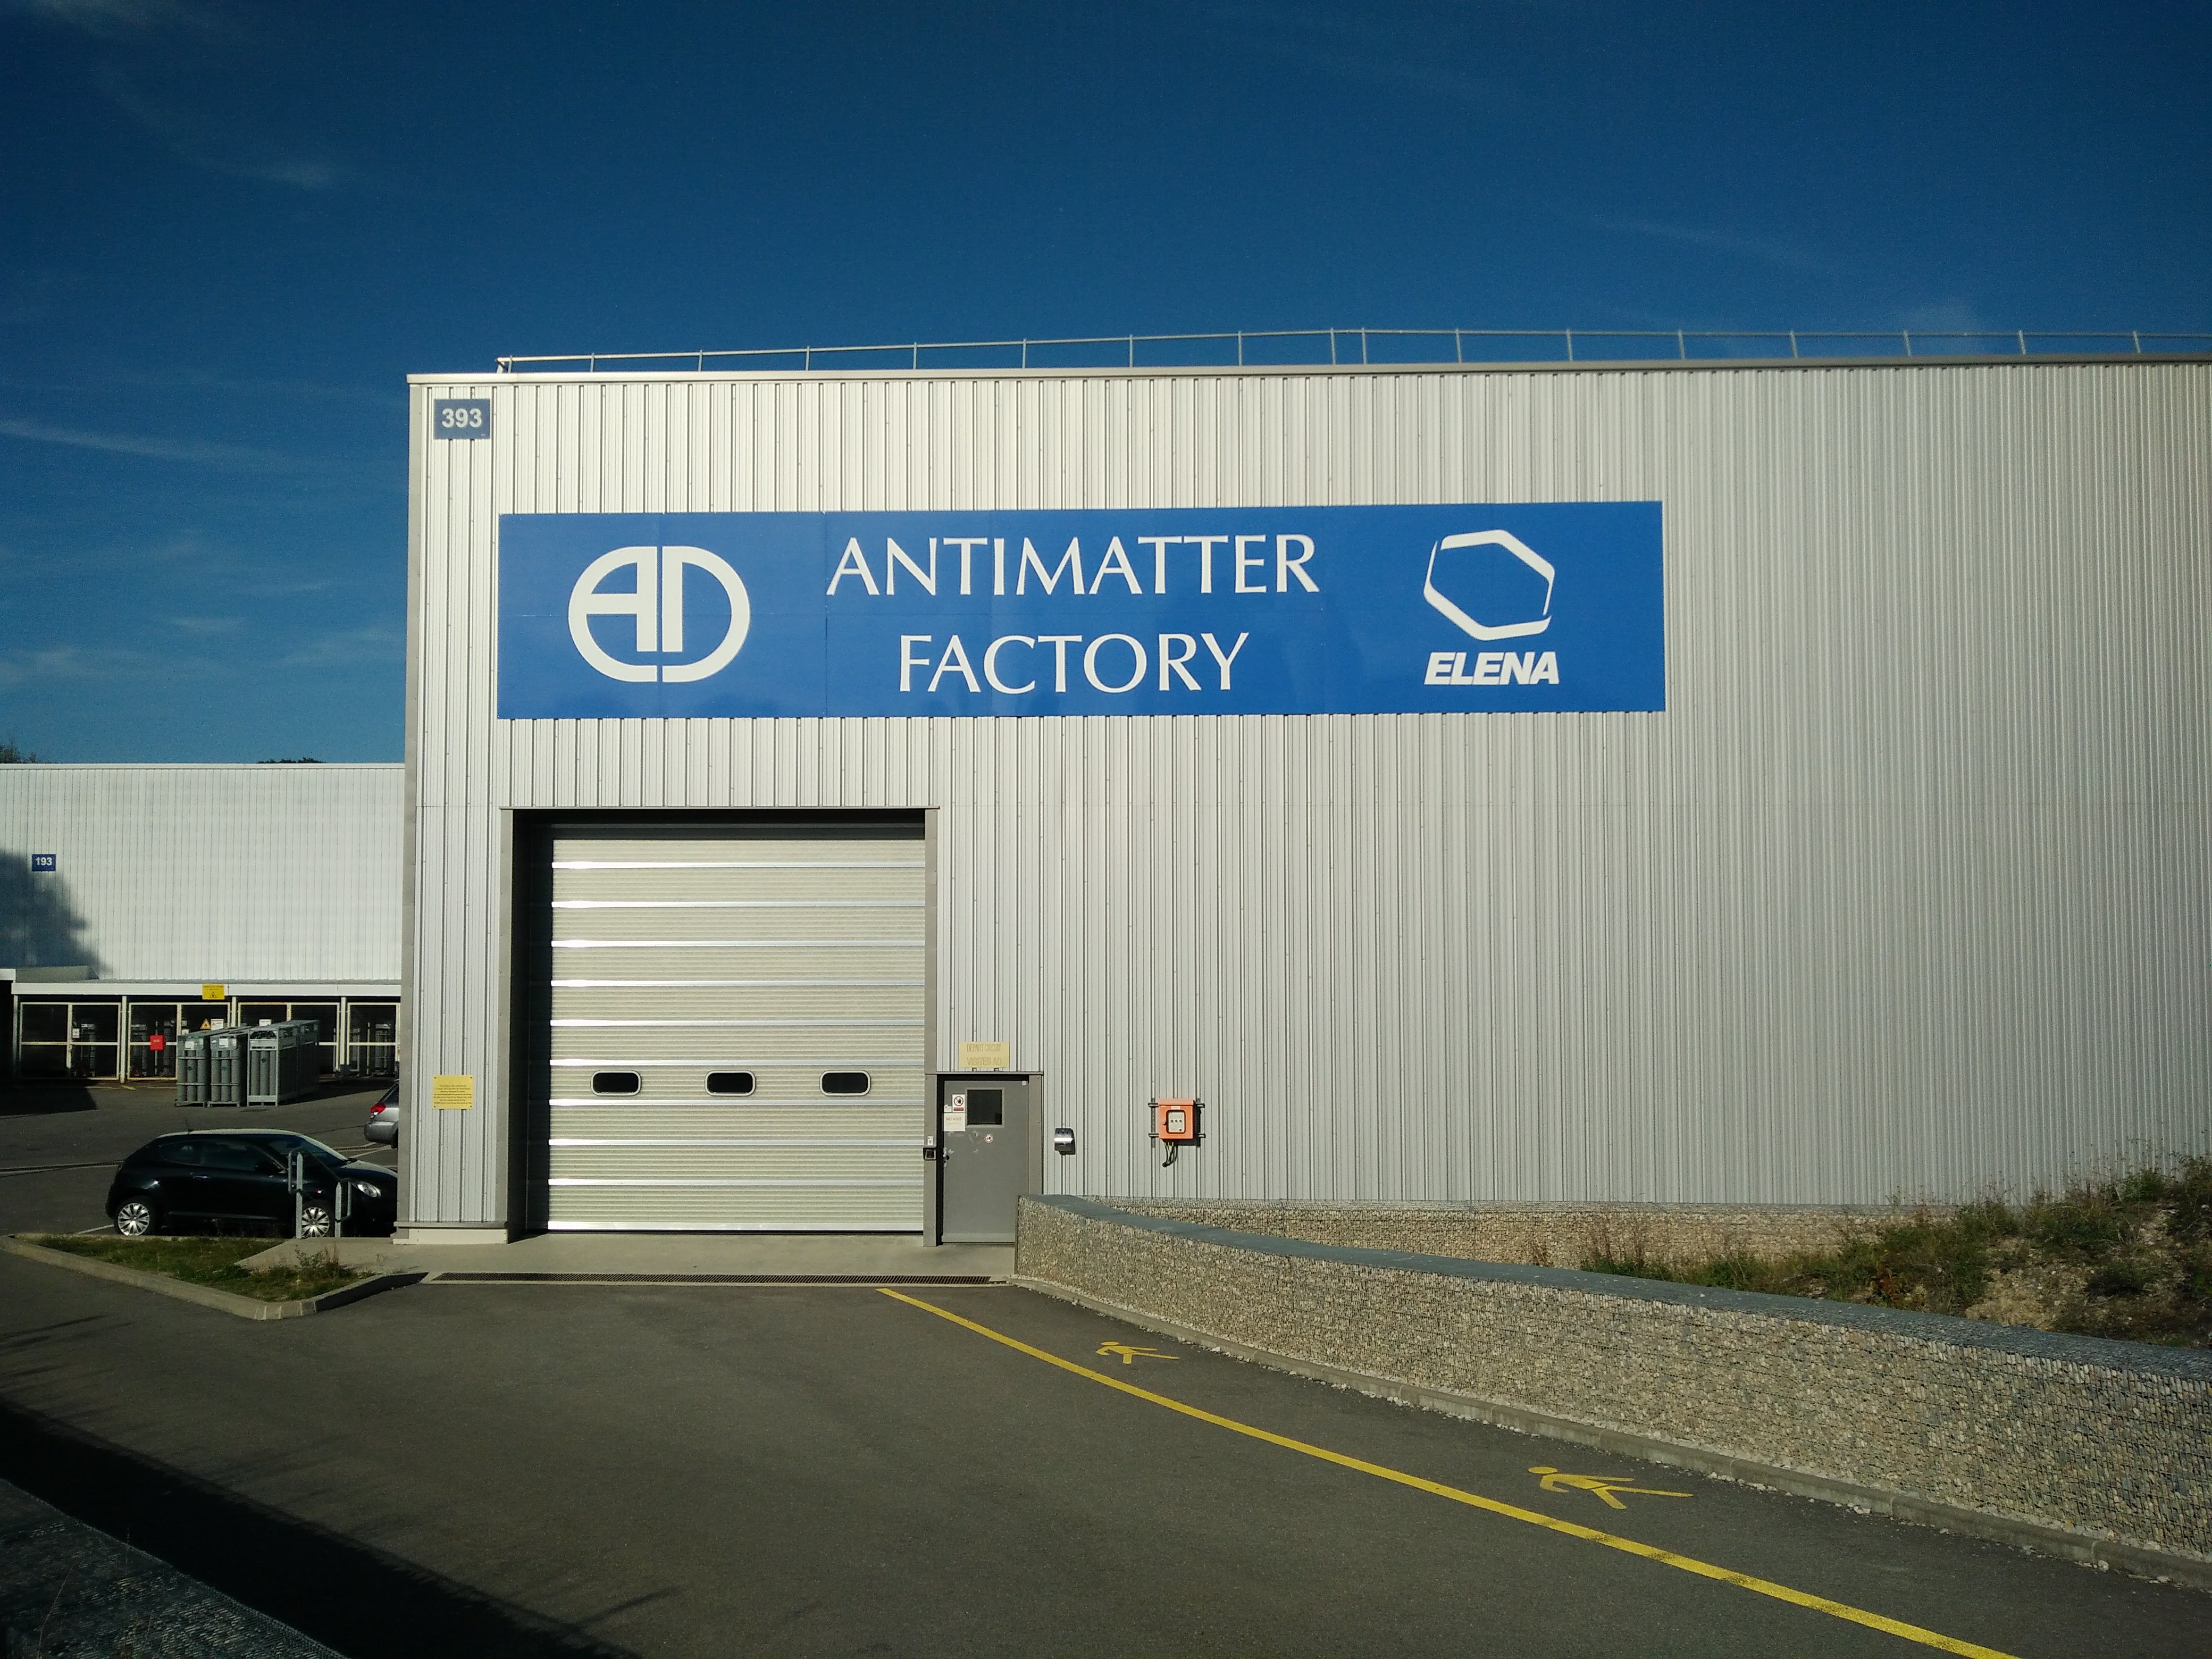
\includegraphics[width=60mm]{antimatter_factory}
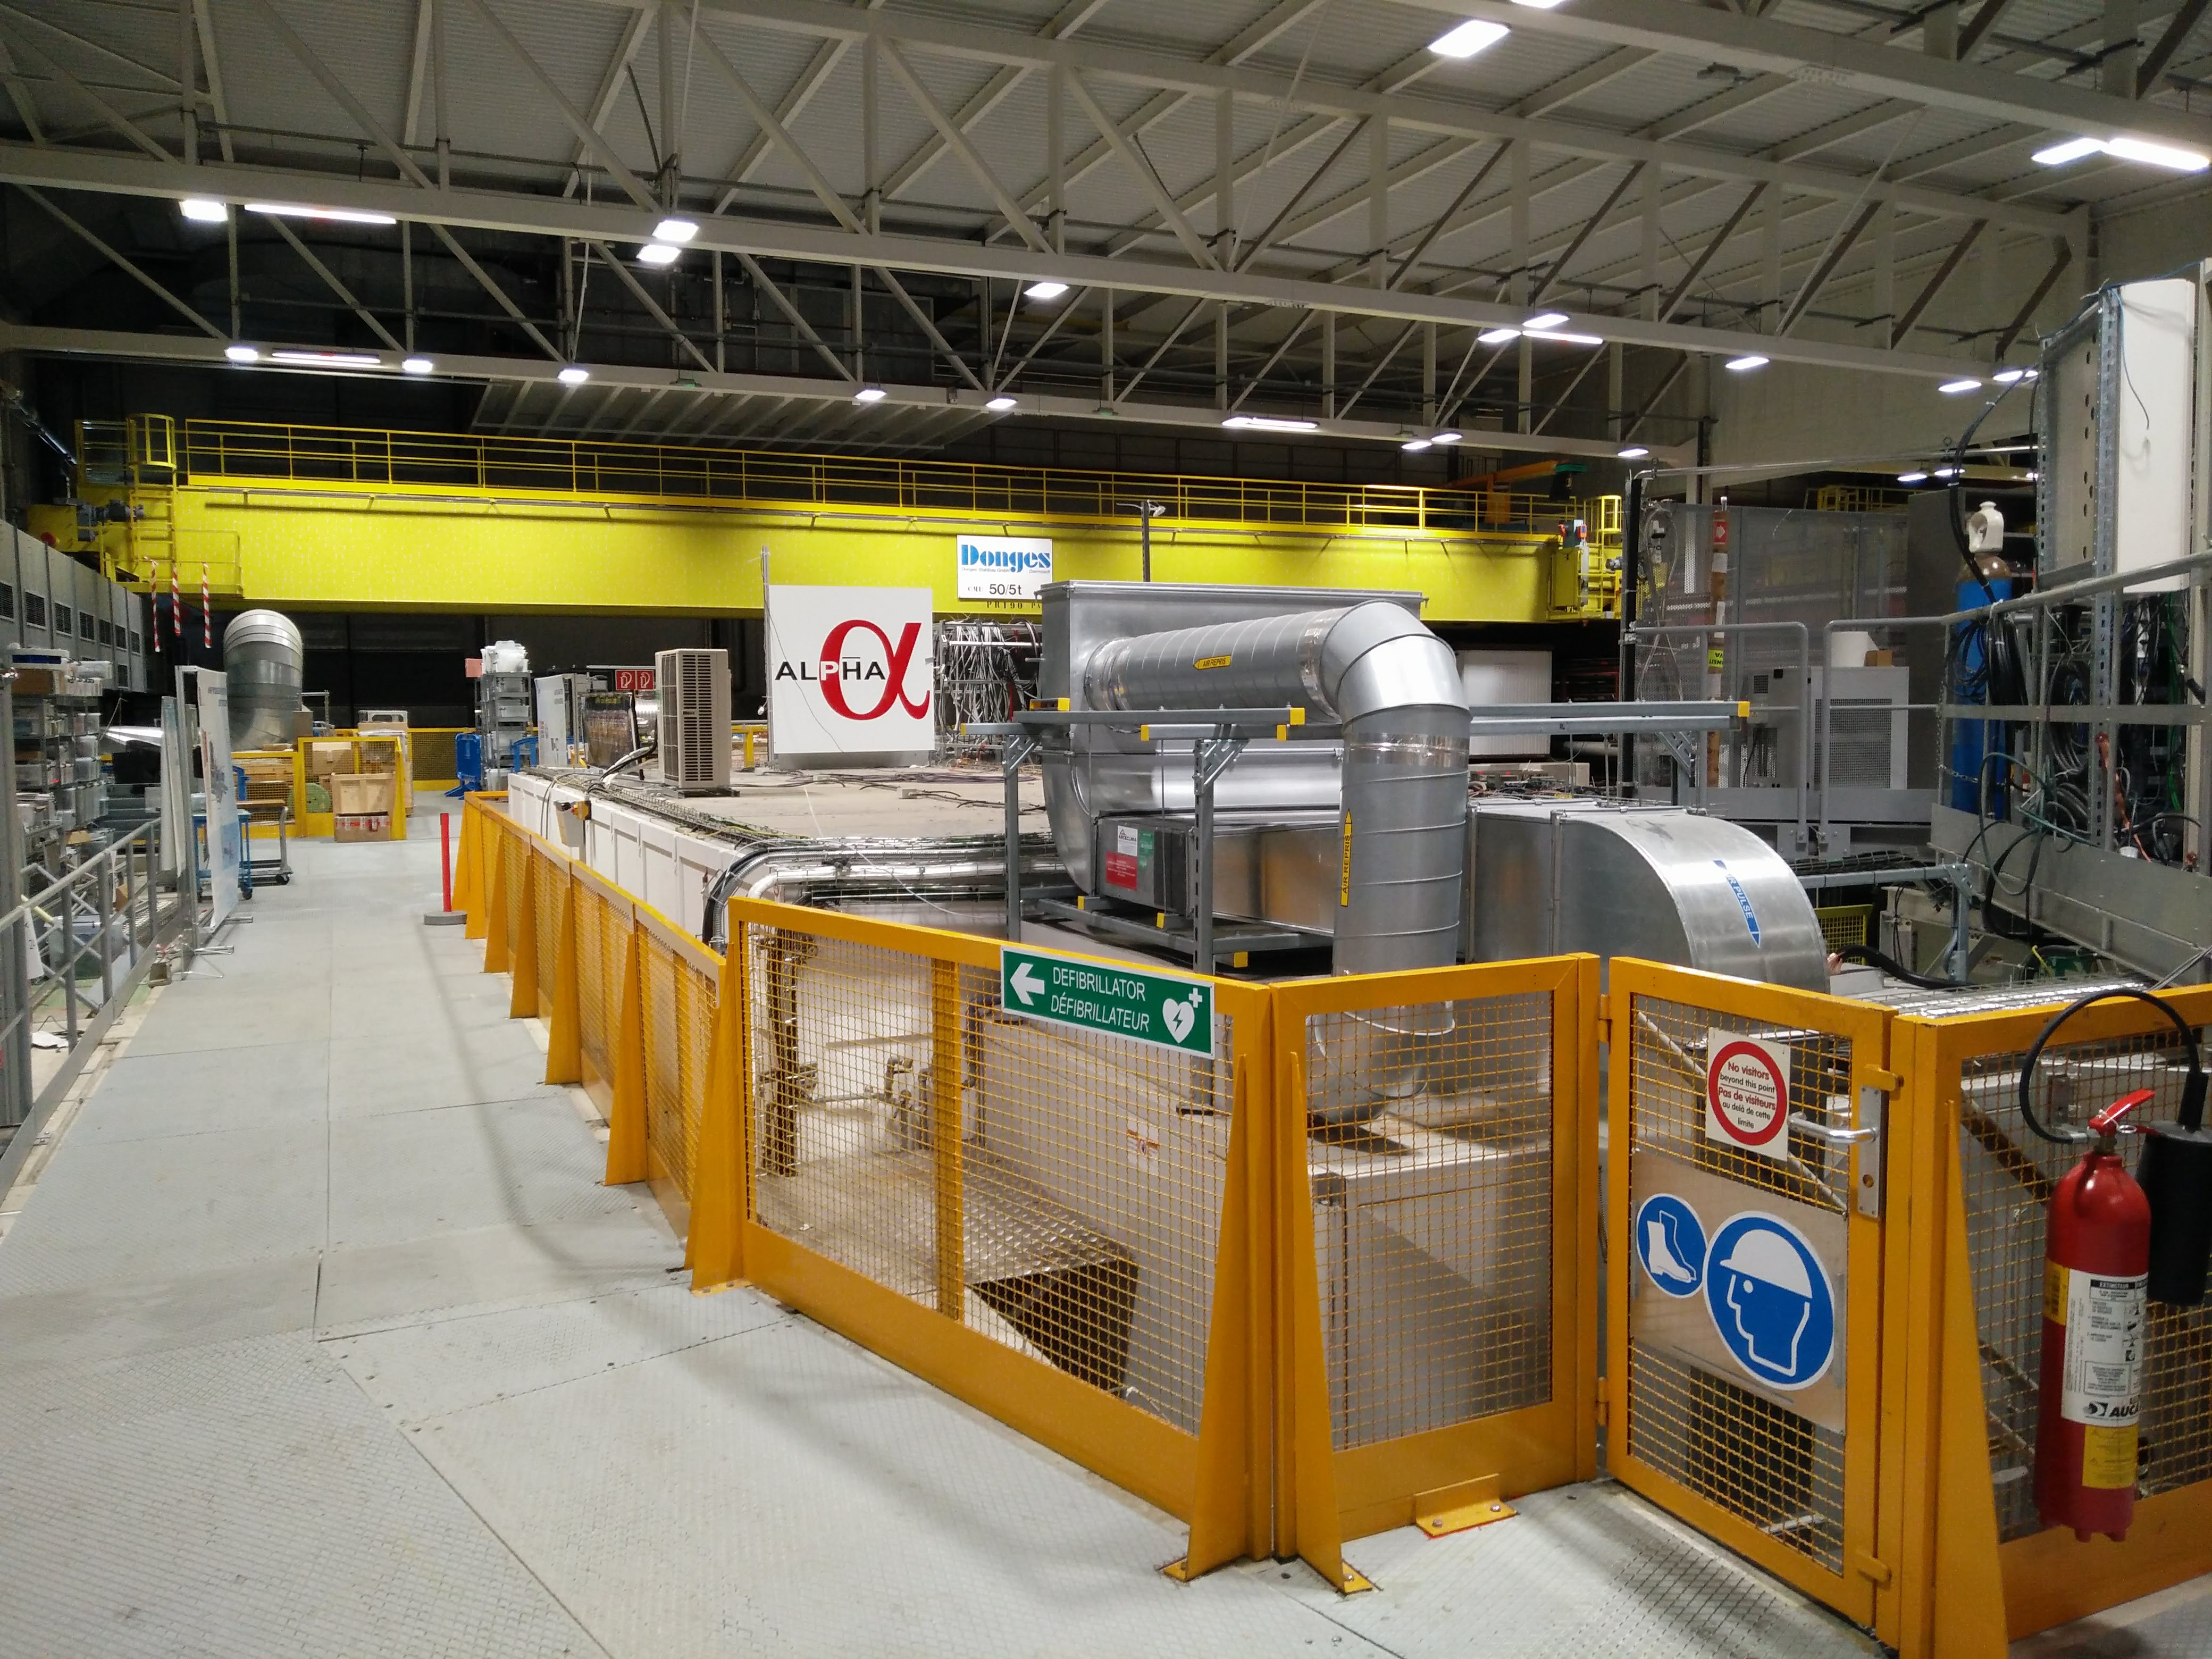
\includegraphics[width=60mm]{alpha_hall}

\caption{Antimatter Factory (left) and ALPHA experiment hall (right)}
\end{figure}

ALPHA has some important components that make the research on antimatters possible. These are: the Penning trap, which holds the positrons and antiprotons before we use them to make antihydrogen, the Atom trap, which traps and holds the antihydrogen atoms, and the Annihilation vertex imaging detector, which detects the antihydrogen atoms when we allow them to annihilate and can find the point at which they annihilated. You can see the full setup of experiment in figure \ref{fig:full_map} .

\begin{figure}[h]
\centering
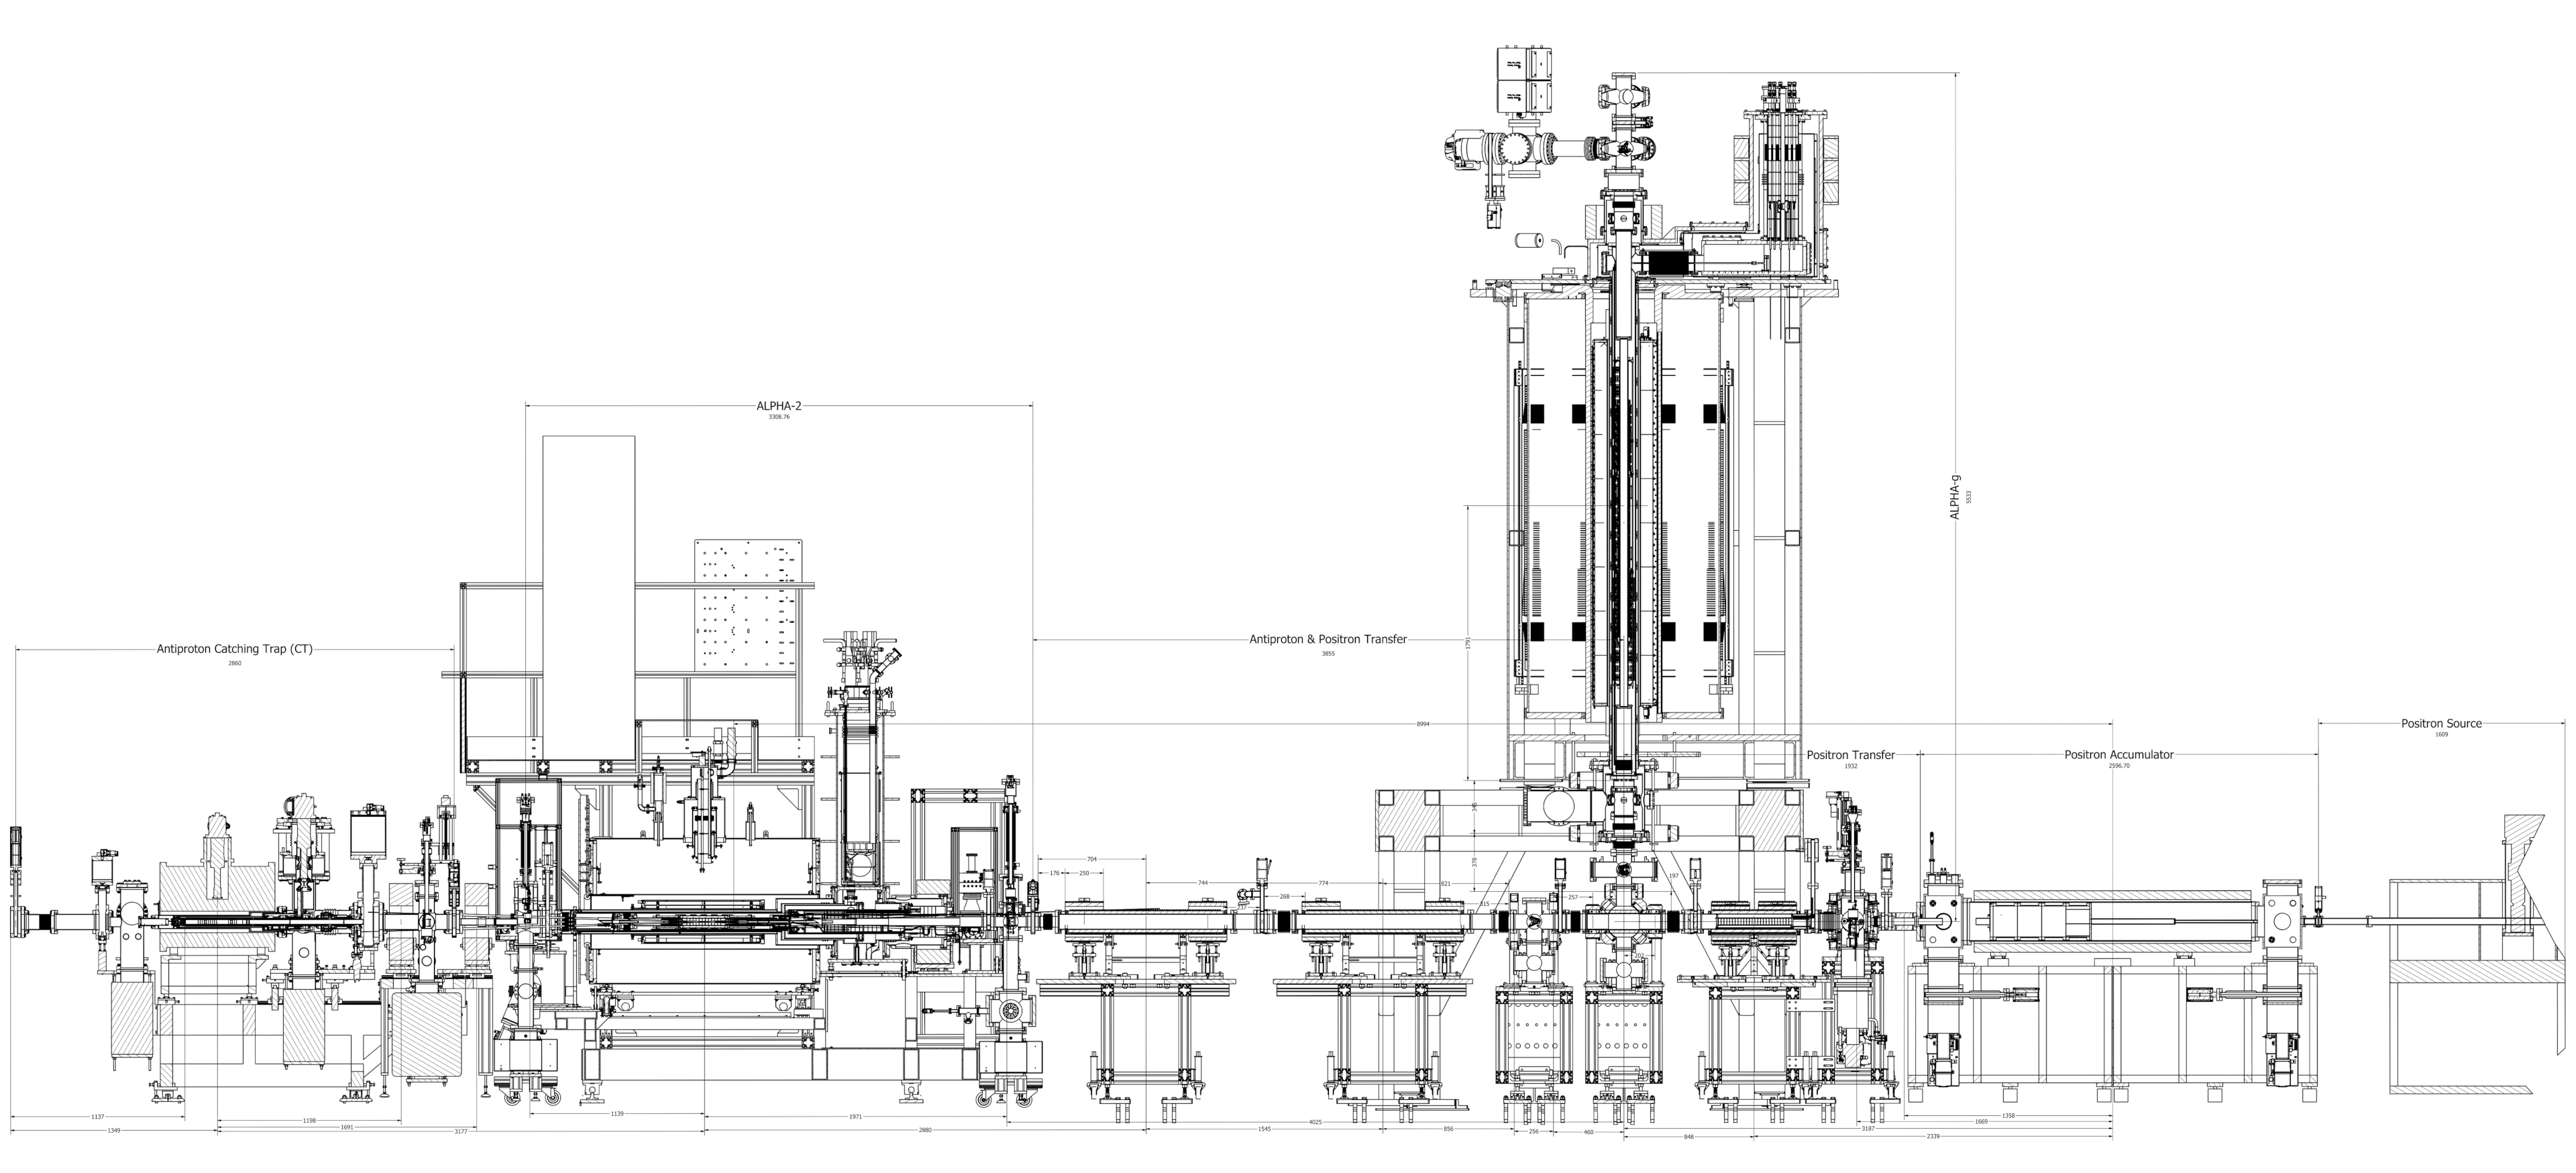
\includegraphics[scale=0.09]{full_map}
\caption{Full Setup of ALPHA experiment}
\label{fig:full_map}
\end{figure}

Note: For pictures in this sections I have used pictures used in web site of ALPHA 
\subsection{Magnets}
\label{Magnets} 
The ALPHA magnetic trap is a variant of the a type of atom trap called an 'Ioffe trap'. This magnetic trap is used to trap antihydrogen atoms which are neutral and electic fields can not be used to trap the particles. Such traps work because most atoms interact with a magnetic field through a property called their magnetic dipole moment. If the atom is moving in a magnetic field, it will gain and lose energy as the strength of the magnetic field near the atom changes. Making a magnetic field that increases in all directions from a central minimum point means that some atoms will gain potential energy and lose kinetic energy if they move away from the minimum. Atoms that have low enough total energy will convert all of their kinetic energy to potential energy and be reflected from higher magnetic field and be trapped. You can think of this like a marble rolling in a bowl -- a slow moving marble can't reach the edge of the bowl and will be `trapped' in the bowl.

\begin{figure}[h]
\centering
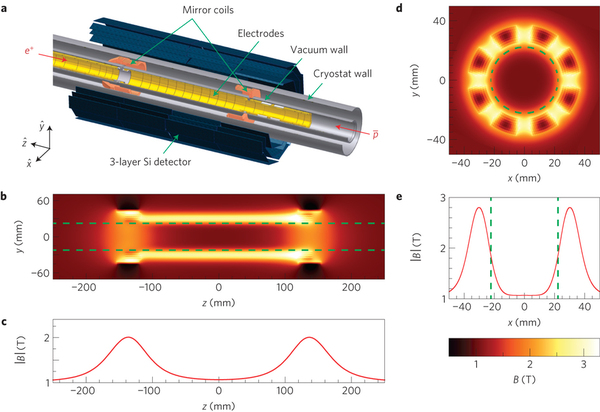
\includegraphics[scale=0.4]{magnets-trap}
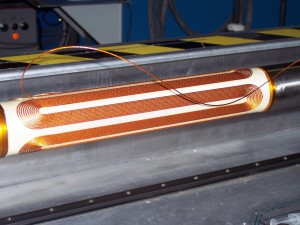
\includegraphics[scale=0.52]{magnet}
\caption{ALPHA Magnetic Trap}
\end{figure}


\subsection{Detectors}
The ALPHA neutral trap is surrounded by a complex particle detector, called the Silicon Vertex Detector (SVD). The SVD could be described as a four megapixel 3D camera, it 'sees' inside the ALPHA -apparatus and is sensitive enough to tell us where and when a single annihilation event occurs. In ALPHA, the antihydrogen atoms annihilate mainly at the gold coated trap walls, but occasionally the annihilation can take place in the vacuum with the tiny amount of residual gas always present in the vacuum systems. The annihilating particles in the ALPHA trap are positron and antiproton. Positron, being a lepton, annihilates with its counterpart, electron, and produces two gamma rays. The annihilation of antiproton is a more complex event, but during the annihilation process several energetic charged particles called pions are emitted. The pions penetrate through the ALPHA -apparatus as well as the SVD, during which a tiny amount of energy is deposited into the three thin silicon sensor layers forming the SVD. The SVD records the locations of these interactions and, using this information, constructs the pion track (helix). As there are several of these tracks, the intersection of the tracks then gives the annihilation spatial location (vertex). In addition to the annihilation events, there is also cosmic muon background the SVD records. The fingerprint of these events, however, is very different from the annihilations and they can be effectively rejected.
\begin{figure}[h]

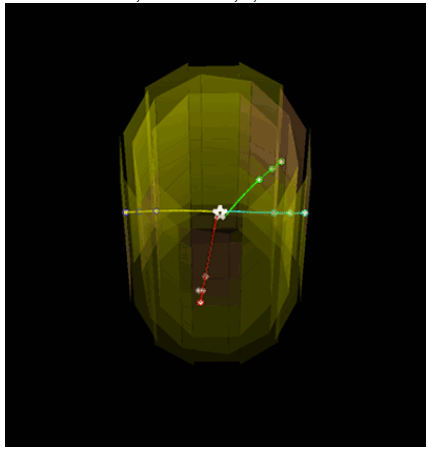
\includegraphics[scale=0.4]{detector}
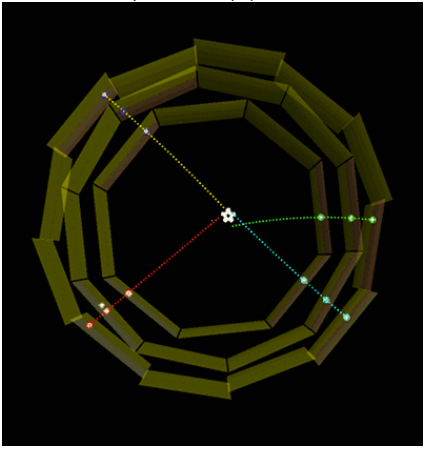
\includegraphics[scale=0.4]{detector-2}
\caption{Silicon Vertex Detector}
\end{figure}


\subsection{Penning trap}
It is a basic and unavoidable fact in the antimatter business that in order to produce antihydrogen, antiprotons and positrons must be mixed. So, ALPHA must have the ability to confine and manipulate charged plasmas with reasonable efficiency and at cryogenic temperatures to boot!
This is accomplished in ALPHA through the use of Penning traps, a type of trap commonly used in plasma physics experiments to confine charged plasmas. Charge is in fact the difference, and indeed the dilemma faced when attempting to trap antihydrogen. Because antihydrogen is neutral, it cannot be held in a traditional Penning trap. This is where ALPHA’s unique magnetic trap comes in (see \ref{Magnets}).

As for positron, antiproton and electron plasmas: a Penning trap will certainly do the trick. In a Penning trap, charged plasmas are confined in a superposition of magnetic and electric fields. You can find a great summary of fields used to trap the particles in figure \ref{trap}
\begin{figure}
\centering

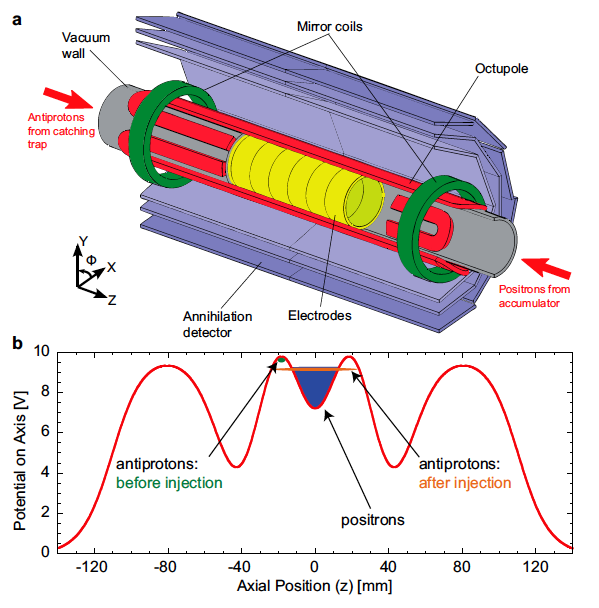
\includegraphics[scale=0.4]{penning-trap-figure}
\caption{Penning Trap}
\label{trap}
\end{figure}

\section{My Projects}
\subsection{Simulation with COMSOL}
When the particles are released from positron source, they trap at the potential valley of the accumulator. Then they release from thr trap to travel toward the pennig trap, which traps the positrons and antiprotons before mixing and making antihydrogen.  positrons, on their way to reach the penning trap, expand because of the space charge. This will make the particles beam larger. So the efficiency of traping positrons at the limited length of penning trap will decrease.


First we decided to see this expansion on simulation. So I set up a simulation with COMSOL and we could see that the standard deviation of particles increases as they travel toward penning trap. because of the long beam line, and the limitation of computational resources I did the simulation in three steps: Short beam line, Long beam line, Real beam line.
\subsubsection{Short Beamline}
In this simulation I set the lenght of beam line to be about 3 meters which only covers the accumulaotr and buncher and I was interested in evaluating the beam shape when they leave the buncher.

The results was quite wired. Because although we could se the pexpansion because of the particle-partilce expansion, but the results was showing a strange decrease at the  stansrad deviation of the z position of the particles. and the decrease in std was getting significent as the the number of particels increased. So I decided to run more simulations with longer beam lines.

\subsubsection{Long Beamline}
In this part of simulation I increased the length of beam line. the size of beam line for these simulations was about 7 meters. 

The significant result of this change was an decrease in the depth of valley at the std(z), and more significant result was time of simulation that increased form 18 hours to 31 hours.
 So we noticed that the valley was because of the end surface of the beam line that as the particles reach there they stick to the surface (this was because of the option that I set in preparing the simulation).
 
\subsubsection{Real Beamline}
this simulatio was very computationaly costly, which took about 23 hours to simulate just five particles. The reults was as we expected. There was no decrease in std(z) of particles. So this simulation was colser to the real setup than perivious ones. So I tryed to simulate the more particles in this setup.

\subsubsection{Buncher Simulation}
As I mentioned earlier, the beam of positrons expand as they travel toward penning trap and this expansion can be supressed using buncher. We need

as we mentione derleite hhgr bhbhu ]uoghrh jfoierj ijre oerhj ojhg ermjoergj ioergi erogj oerjrhg iergj reiomoghereoimgnoerh gioerjogj remig rej goig erjmgoigh erjgh erjgngreh mgjnererhg rejerrg ermjgngre jmgerger jmernggfjerj nffh rejnhgg ermngoieghr gjmerjhg ermnegre jgnregh ermngbernkljggh erjmgnhgjmeirgergjmmgerhmjgier ifergijer gjoerio gjren ger giejrerr geir gierg ererg erioingg ering erno greonh erong erg eboherg borenij gjre jrenoff erno rieno frenoi freuohf rnoeh fenof renofnrn ejnofrunnr enih9freno feo
g
\subsection{LabVIEW Interface}
Advanced and complicated Experiments like most of the experimenst at cern, are impossible without using the advanced electronics for both collecting and analyzing data and controling the experiment apartues. For these advanced experinents there are tons of parameters to be controled, which are done in the control room (figure \ref{control}). 
So having a safe and graphical interface for this purpose has a key rule. In this project I desinged a safe and graphical interface to control the positron source. 

\begin{figure}[h]
\centering
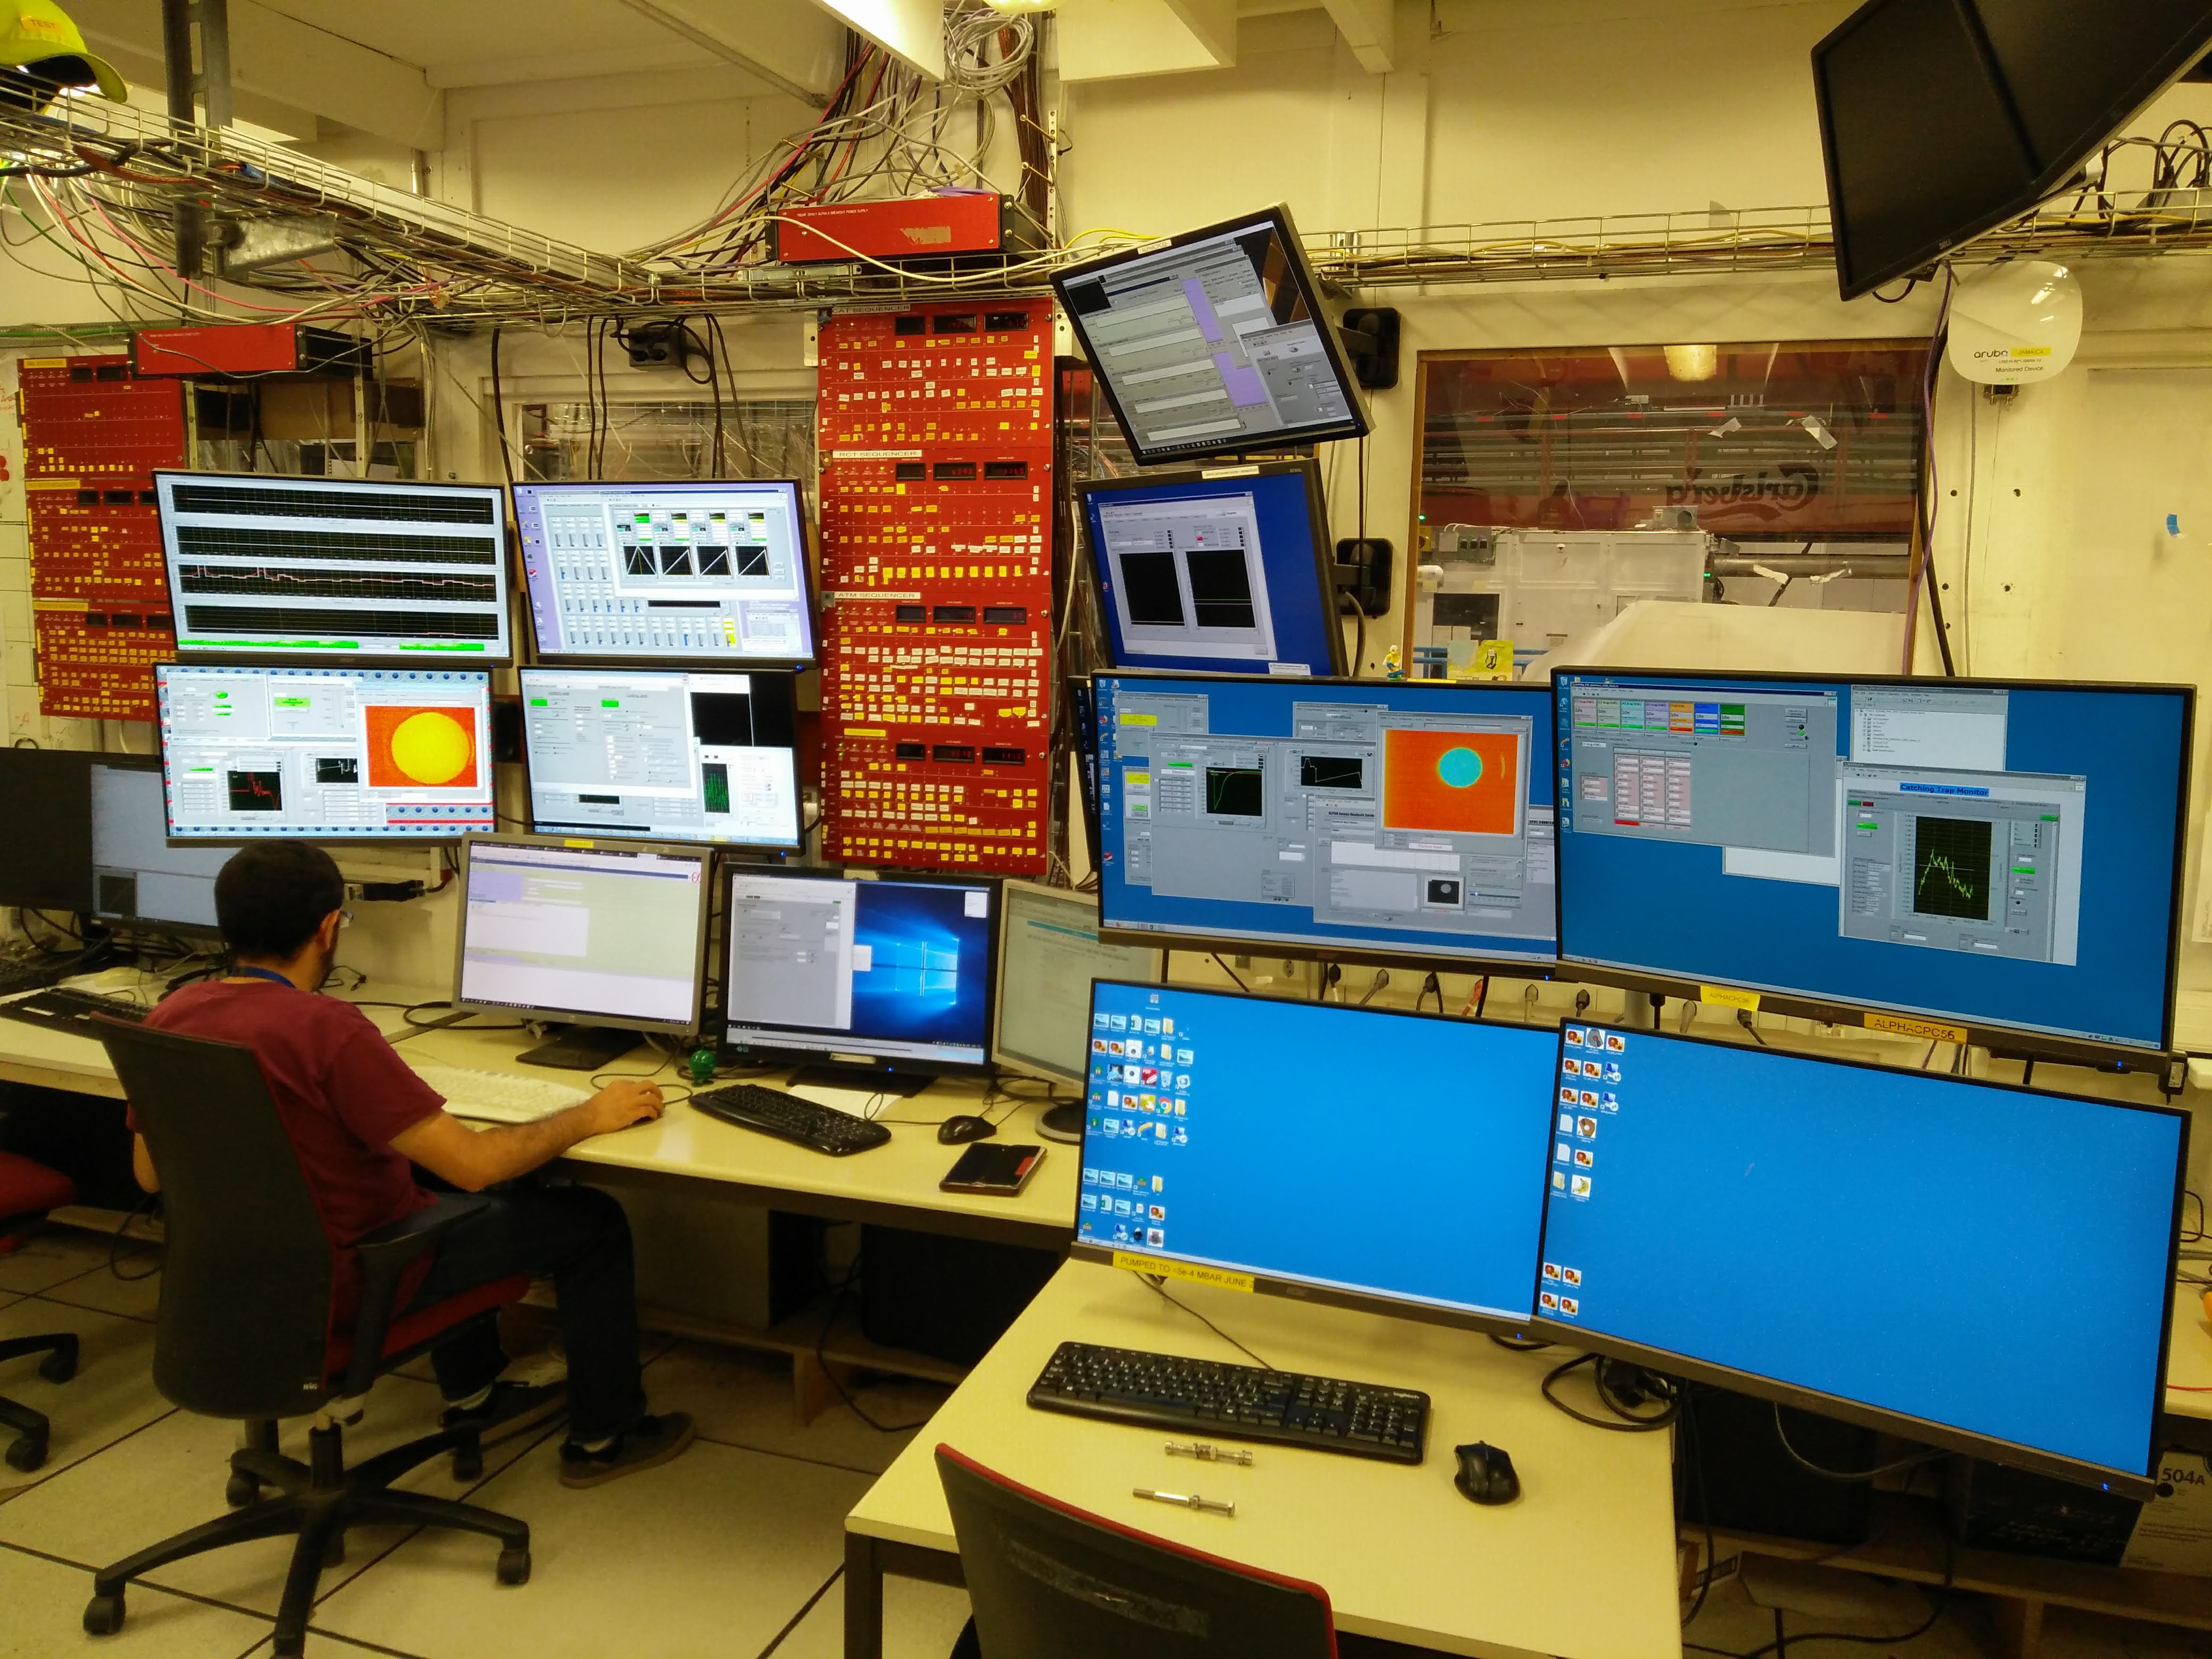
\includegraphics[scale=0.082]{control_room}
\caption{Control Room}
\label{control}
\end{figure}




\subsubsection{Positron Source aparues}

ALPHA derives its positrons from a radioactive beta-decay source containing an isotope of sodium, Na-22. This isotope, which has a conveniently long half-life of about 2.6 years, emits positrons with a large spread of kinetic energies up to about 545 keV. Such energetic positrons cannot easily be applied for antihydrogen production, so that ALPHA uses a well established technique to produce a low energy (eV) beam of positrons in vacuum.

Positrons implanted into solid material typically have a lifetime less than one nanosecond, a thousand millionth of a second. However, during that brief time most will slow down by a variety of energy loss processes to reach kinetic energies close to those characteristic of the temperature of the solid. This process is termed moderation, as the positron’s kinetic energy is lowered, or moderated. Whilst most of the positrons penetrate deep into the bulk of the material and annihilate there, about 1 percent
 stop close enough to the surface that they can diffuse back to it before they annihilate. Incredibly, most of the positrons which reach the surface are emitted into vacuum at low energy, and can be readily formed into a beam and transported, typically using magnetic guiding fields. ALPHA uses a solid film of condensed neon as its moderator; this is one of the most efficient positron moderators.
 
 
\begin{figure}[h]
\centering
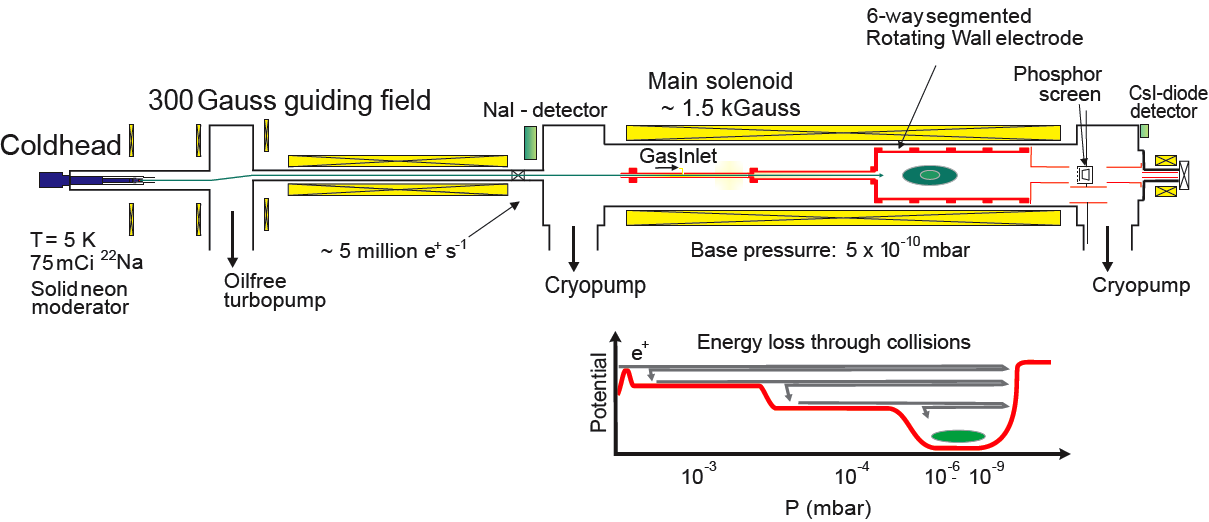
\includegraphics[width=130 mm]{fullsetup}
\caption{Positron Source and Accumulator}
\end{figure}

\subsubsection{Experiment Control}

The computers that controls the different parameters of setup are held by [sotoons] held on the control platforms (figure \ref{platform}). 


\begin{figure}[h]

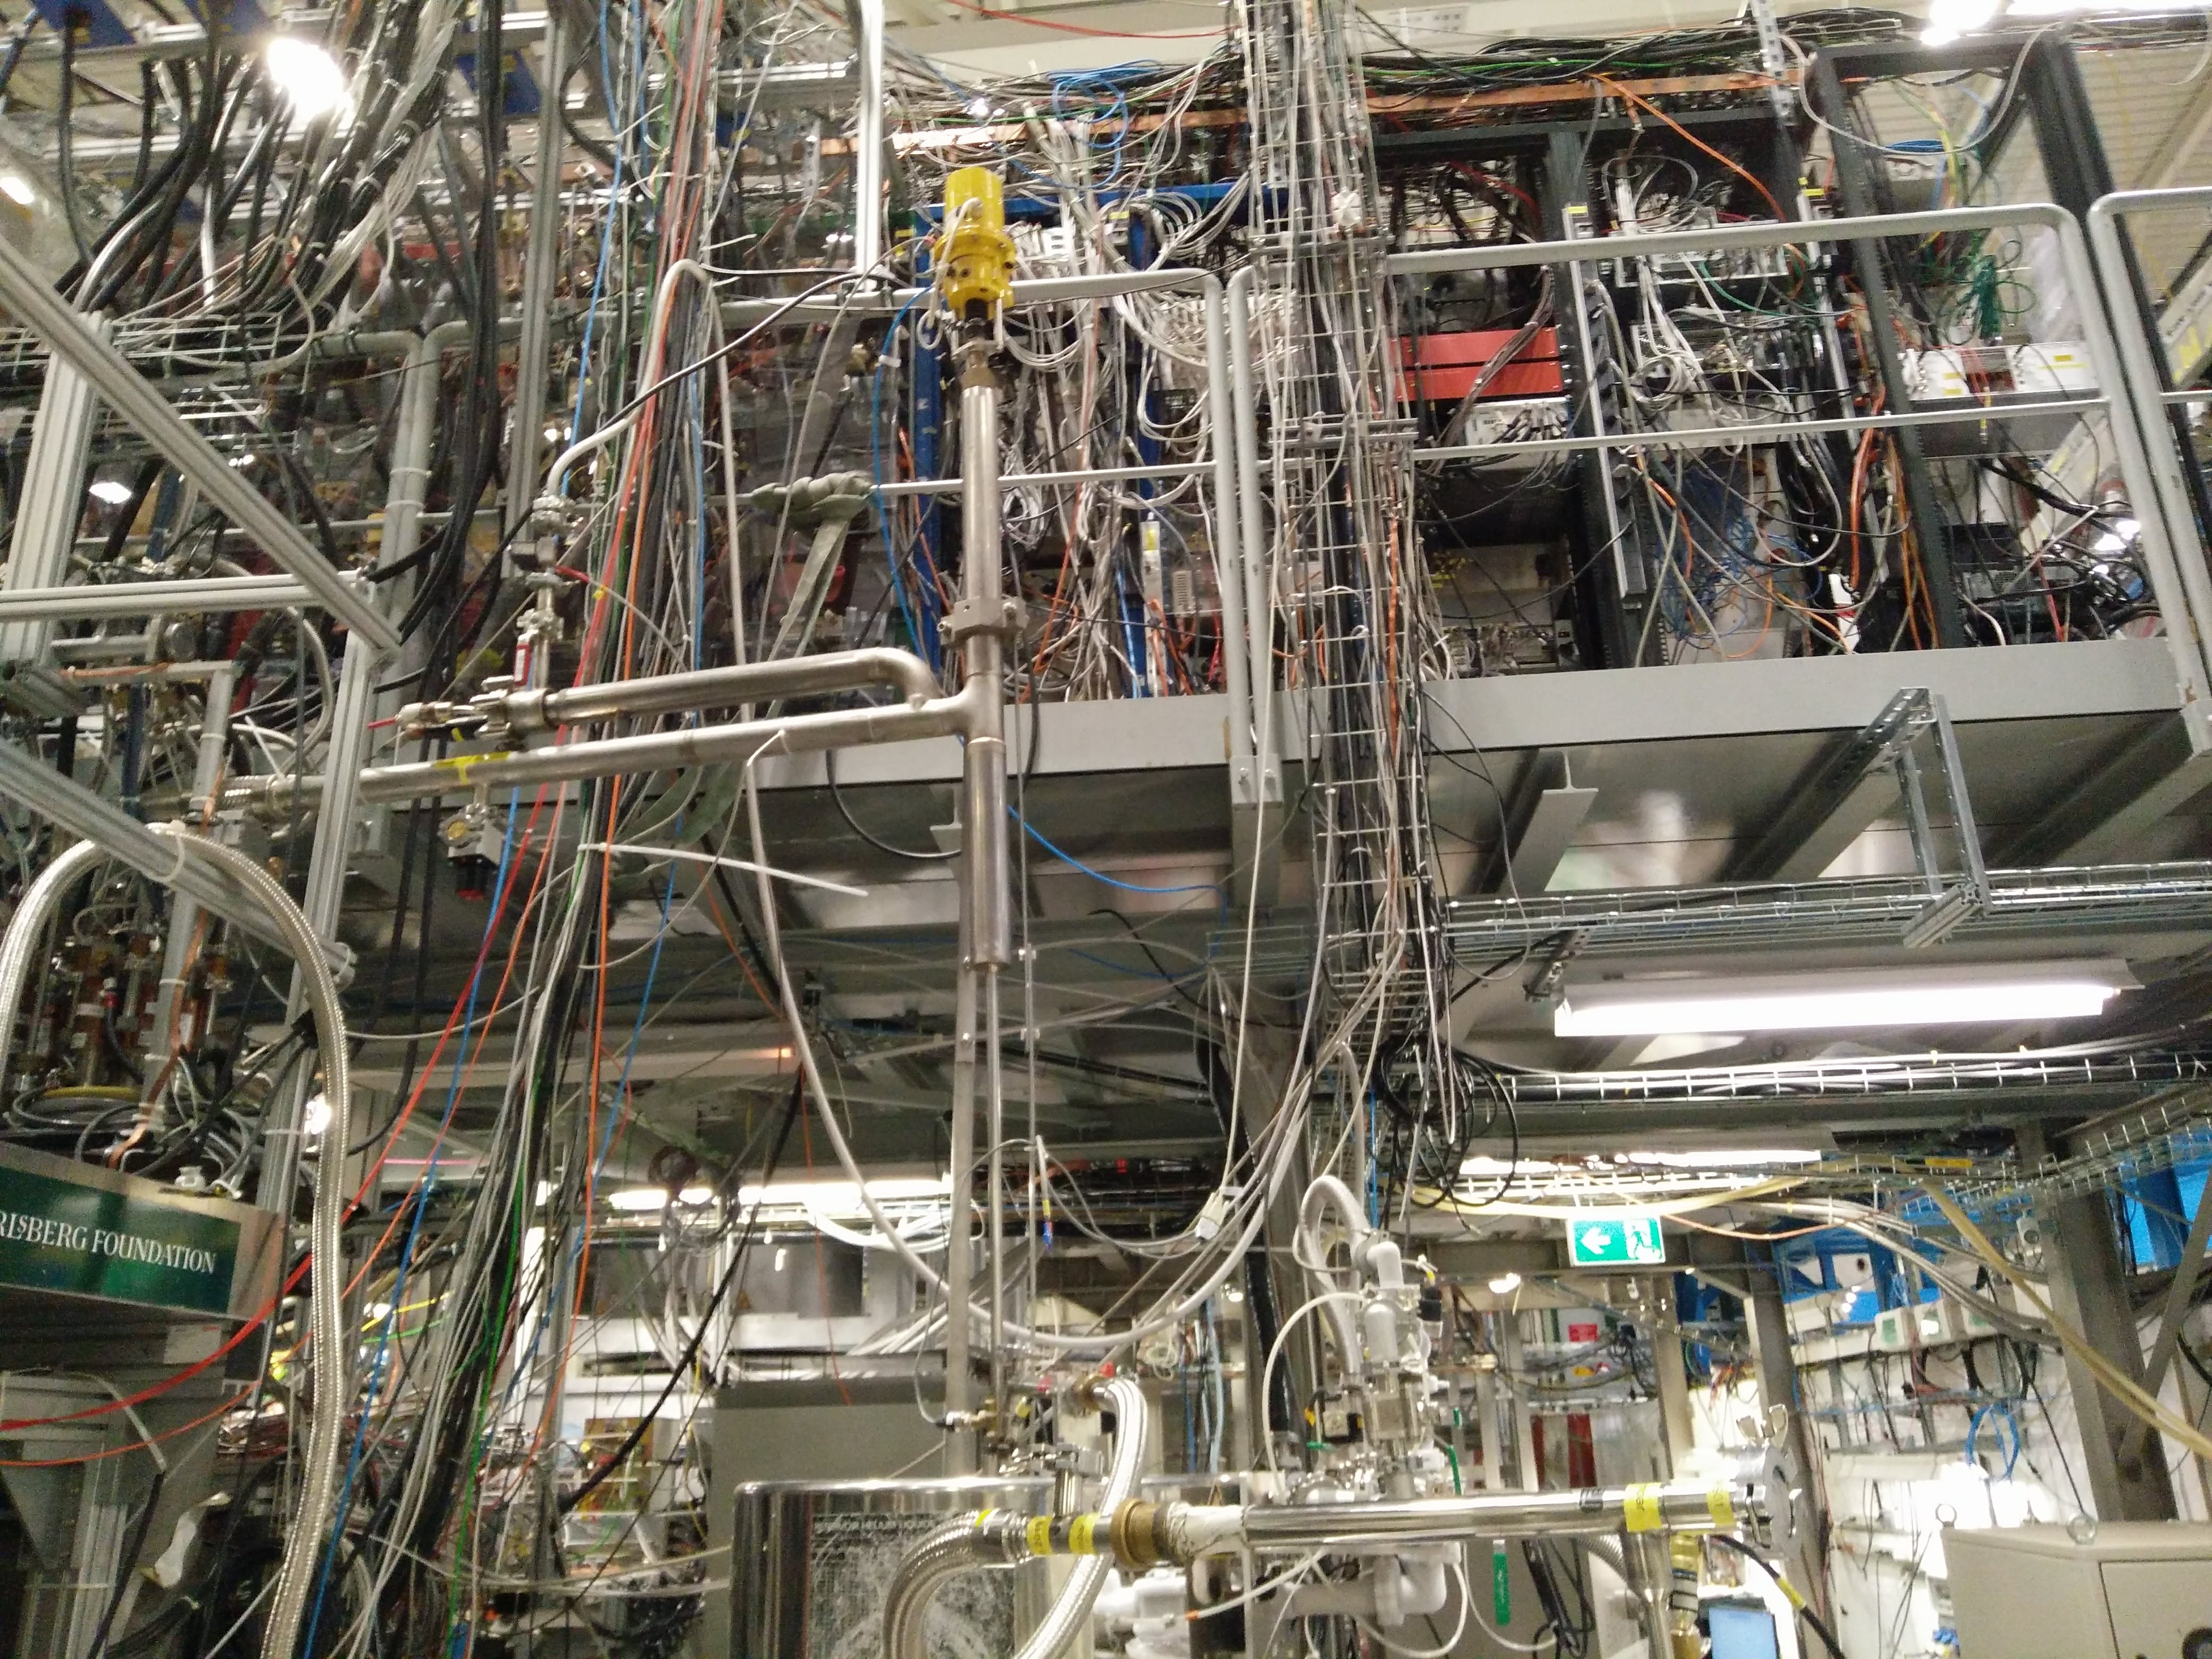
\includegraphics[height=60mm, width=75mm]{control_platform-1}
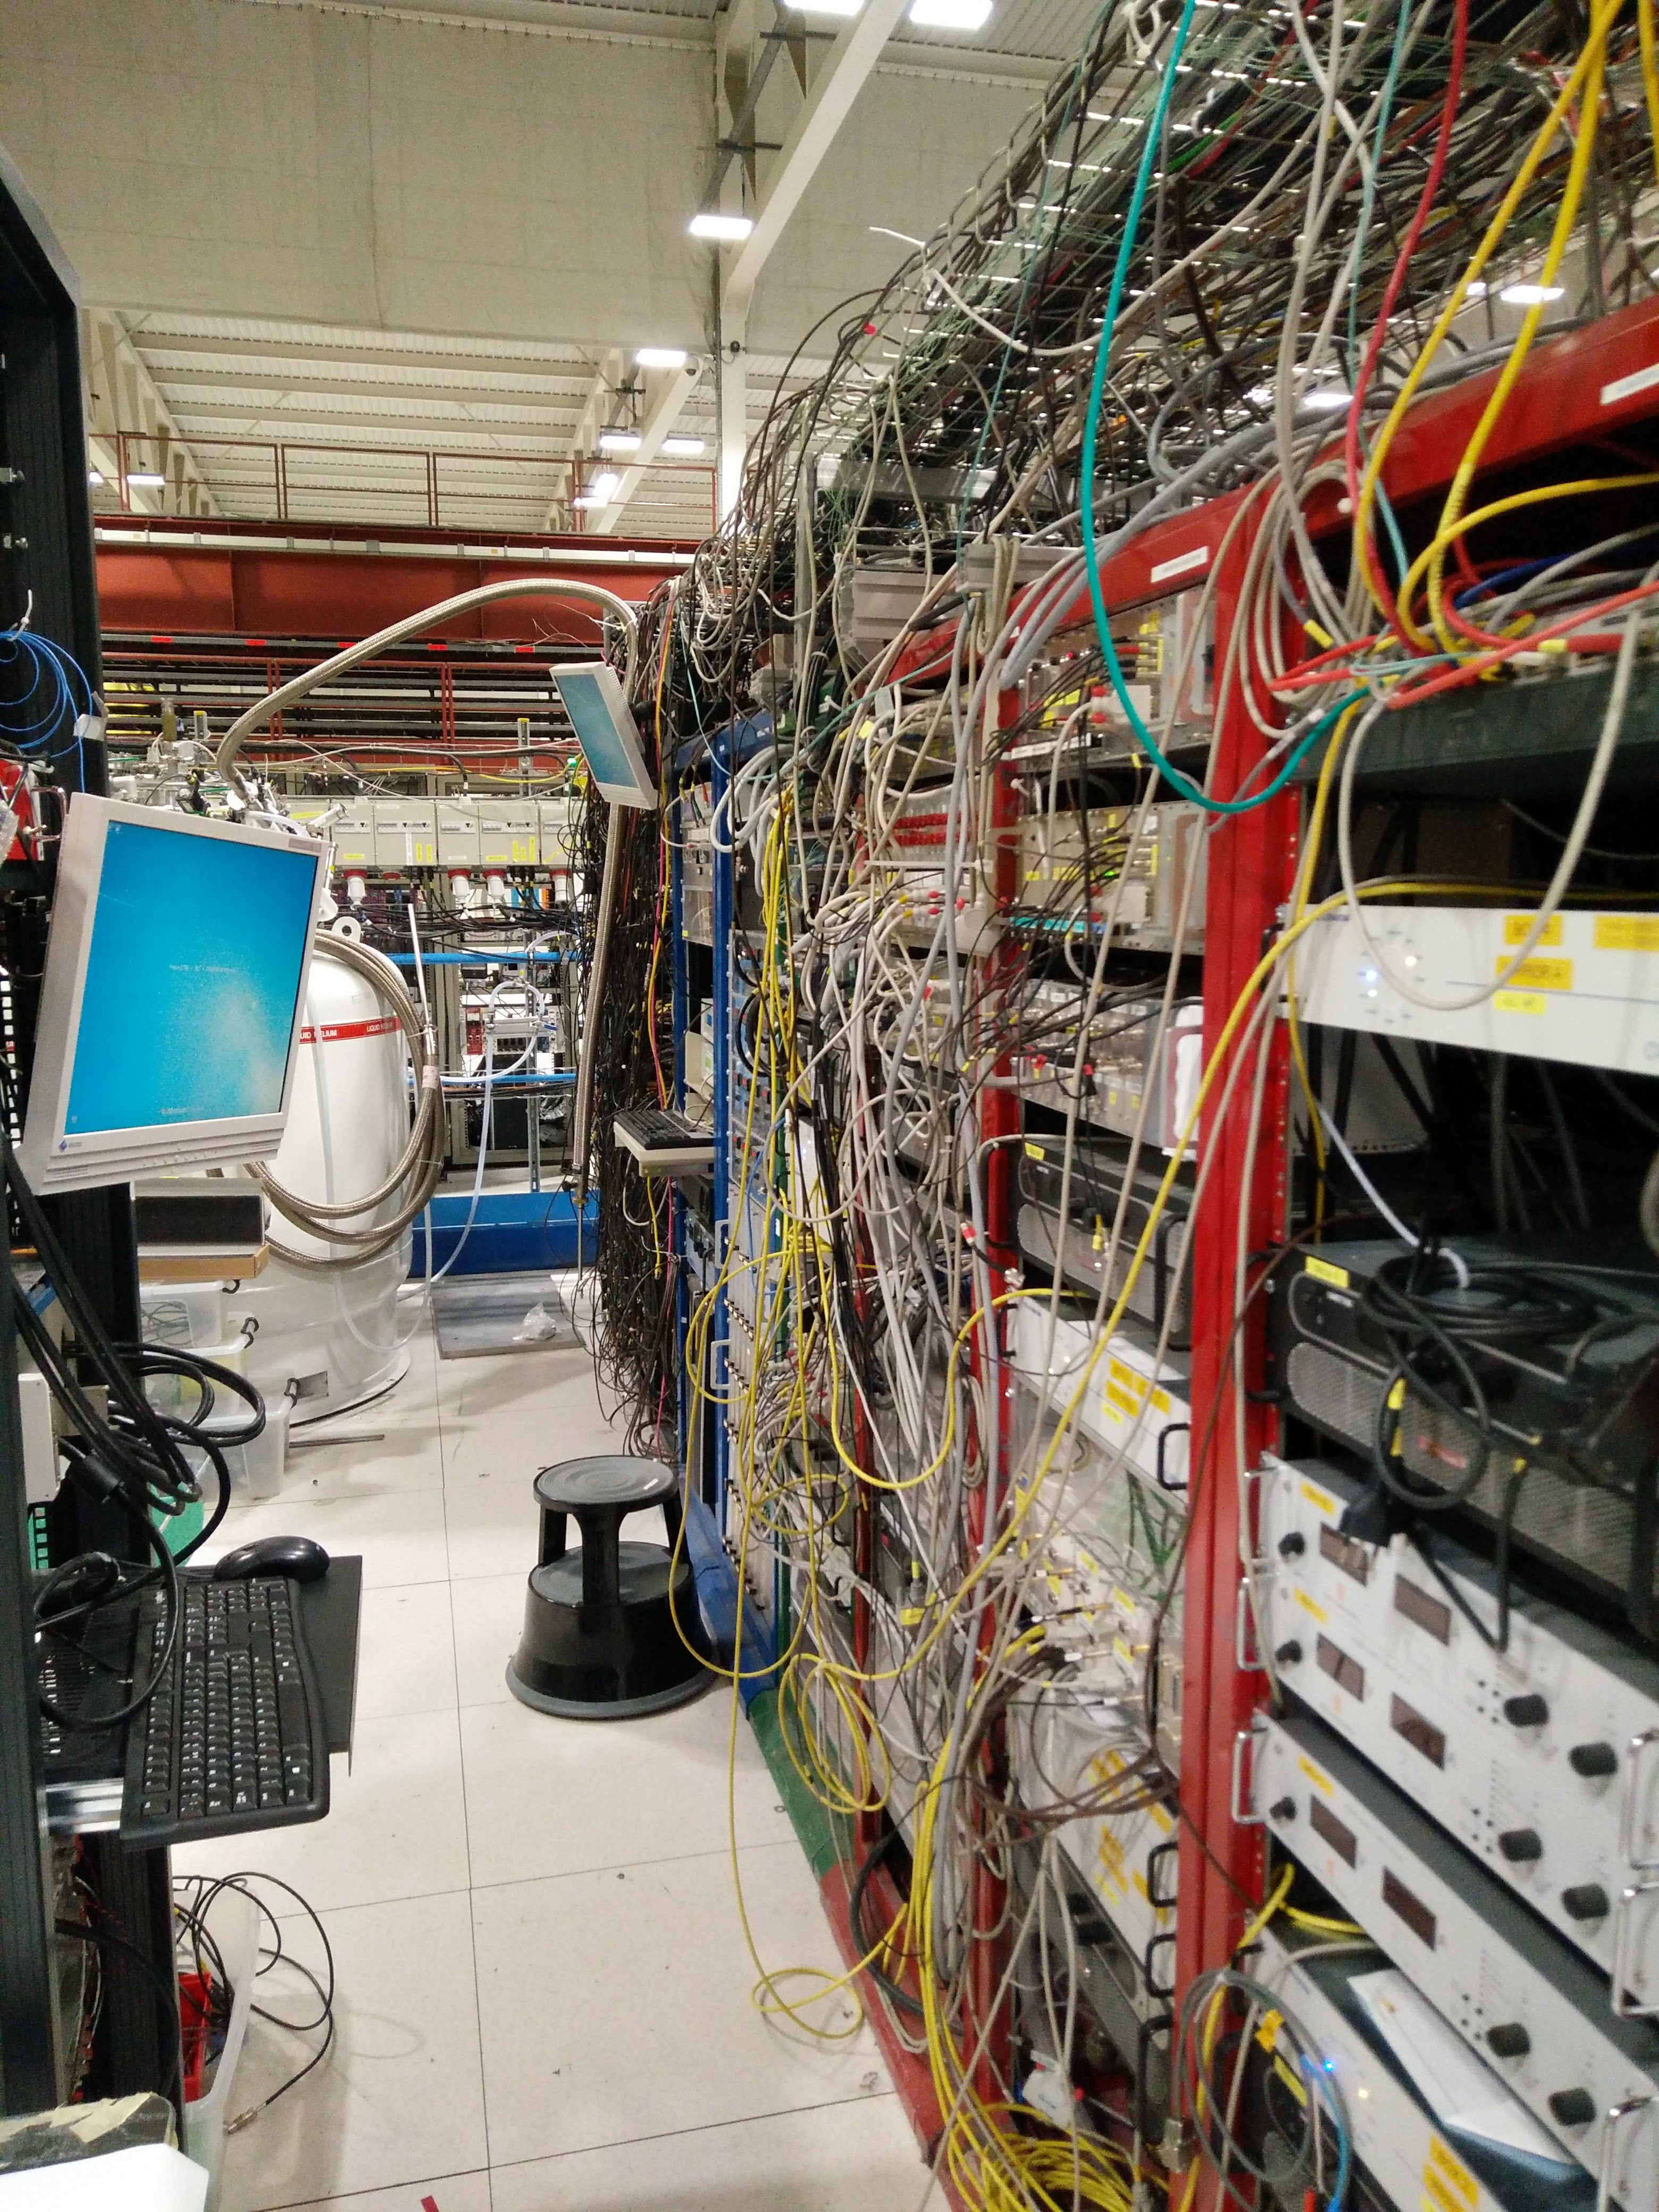
\includegraphics[width=45mm]{control_plattform2}
\caption{Control Platform}
\label{platform}
\end{figure}		
	
All of this computers has special cards installed on their motherboards ( for example NI PCI-6229 for analog inputs, NI PCI-6713 for analof outputs, NI PCI-8431 for RS 485 communications, NI PCI-8430 for RS 232 communication and many other cards). The user can control the experiment throught these cards. The analog and digital signals which indicates the state of individual parts on experiment setup, are collected by the input gates. Then by evaluationg the signals in control room proper signal is send by output gates to the experiment components (like vaccum pumps, valves, current of magnets, electric potential on electrodes, etc).

\begin{figure}[h]
\centering
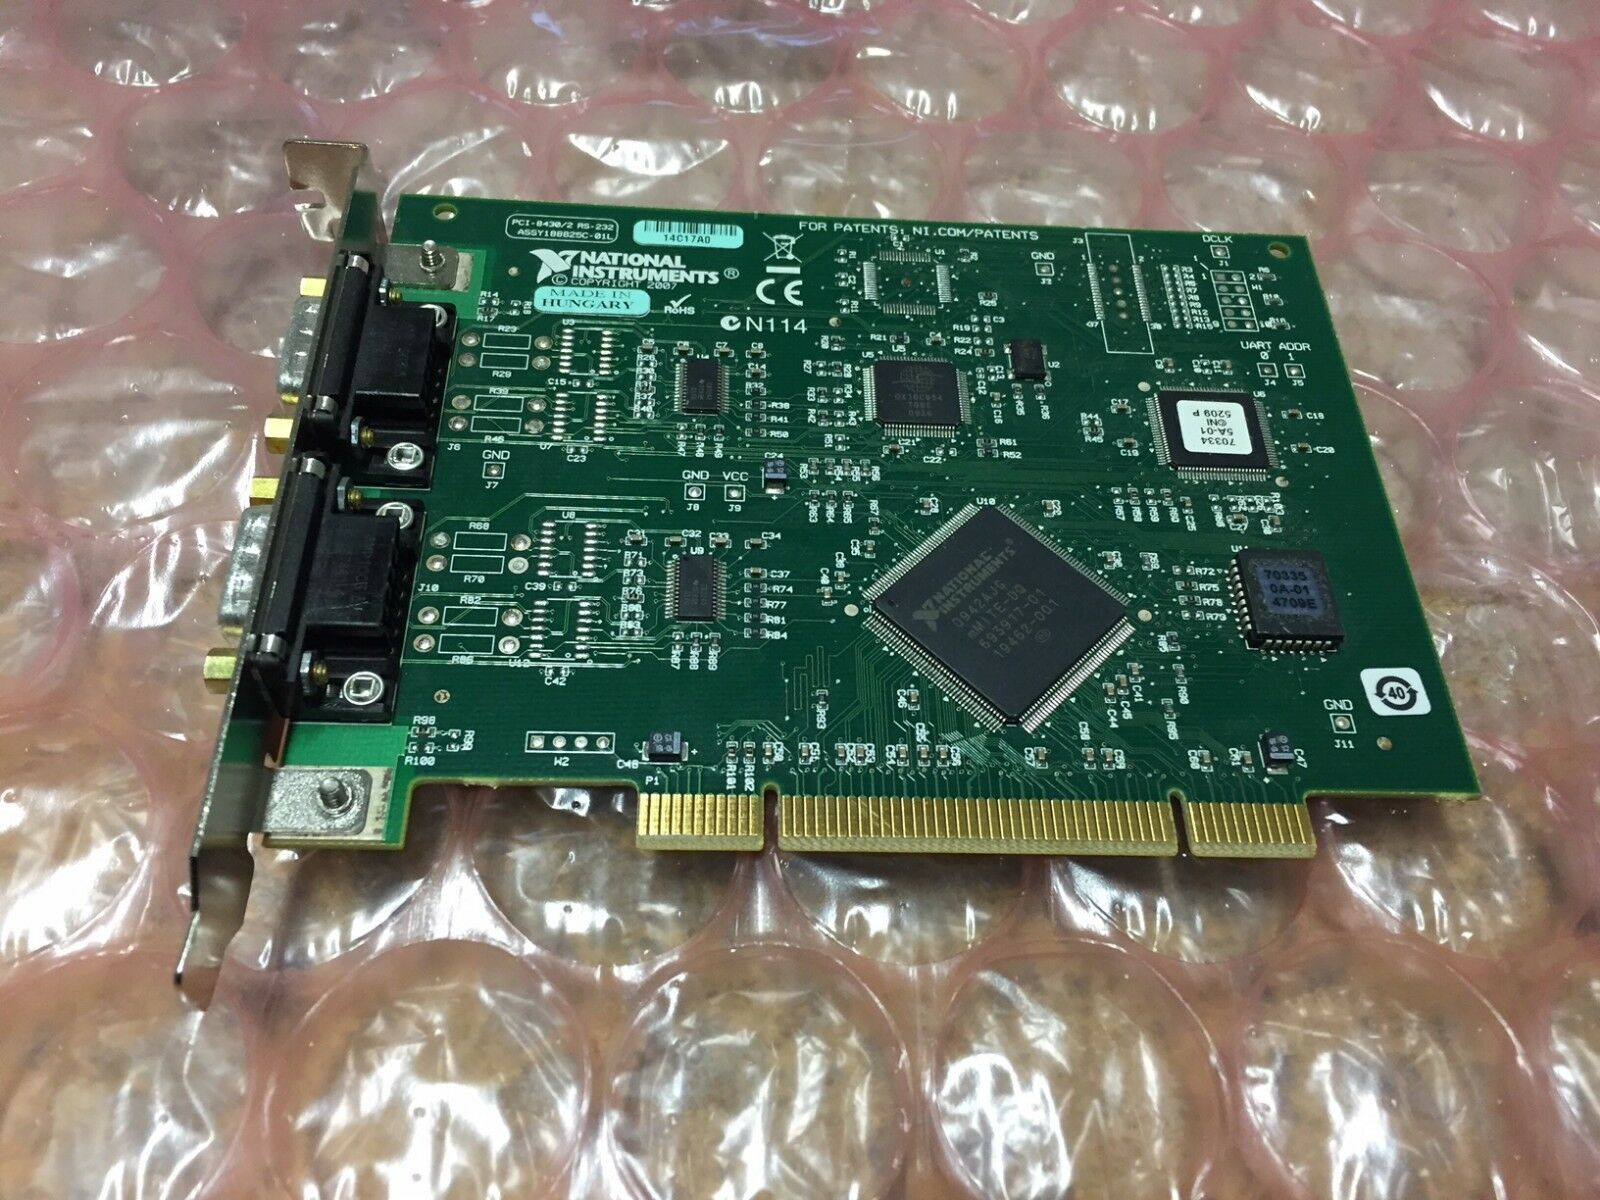
\includegraphics[width=40mm, height=50mm]{PCI_8430}
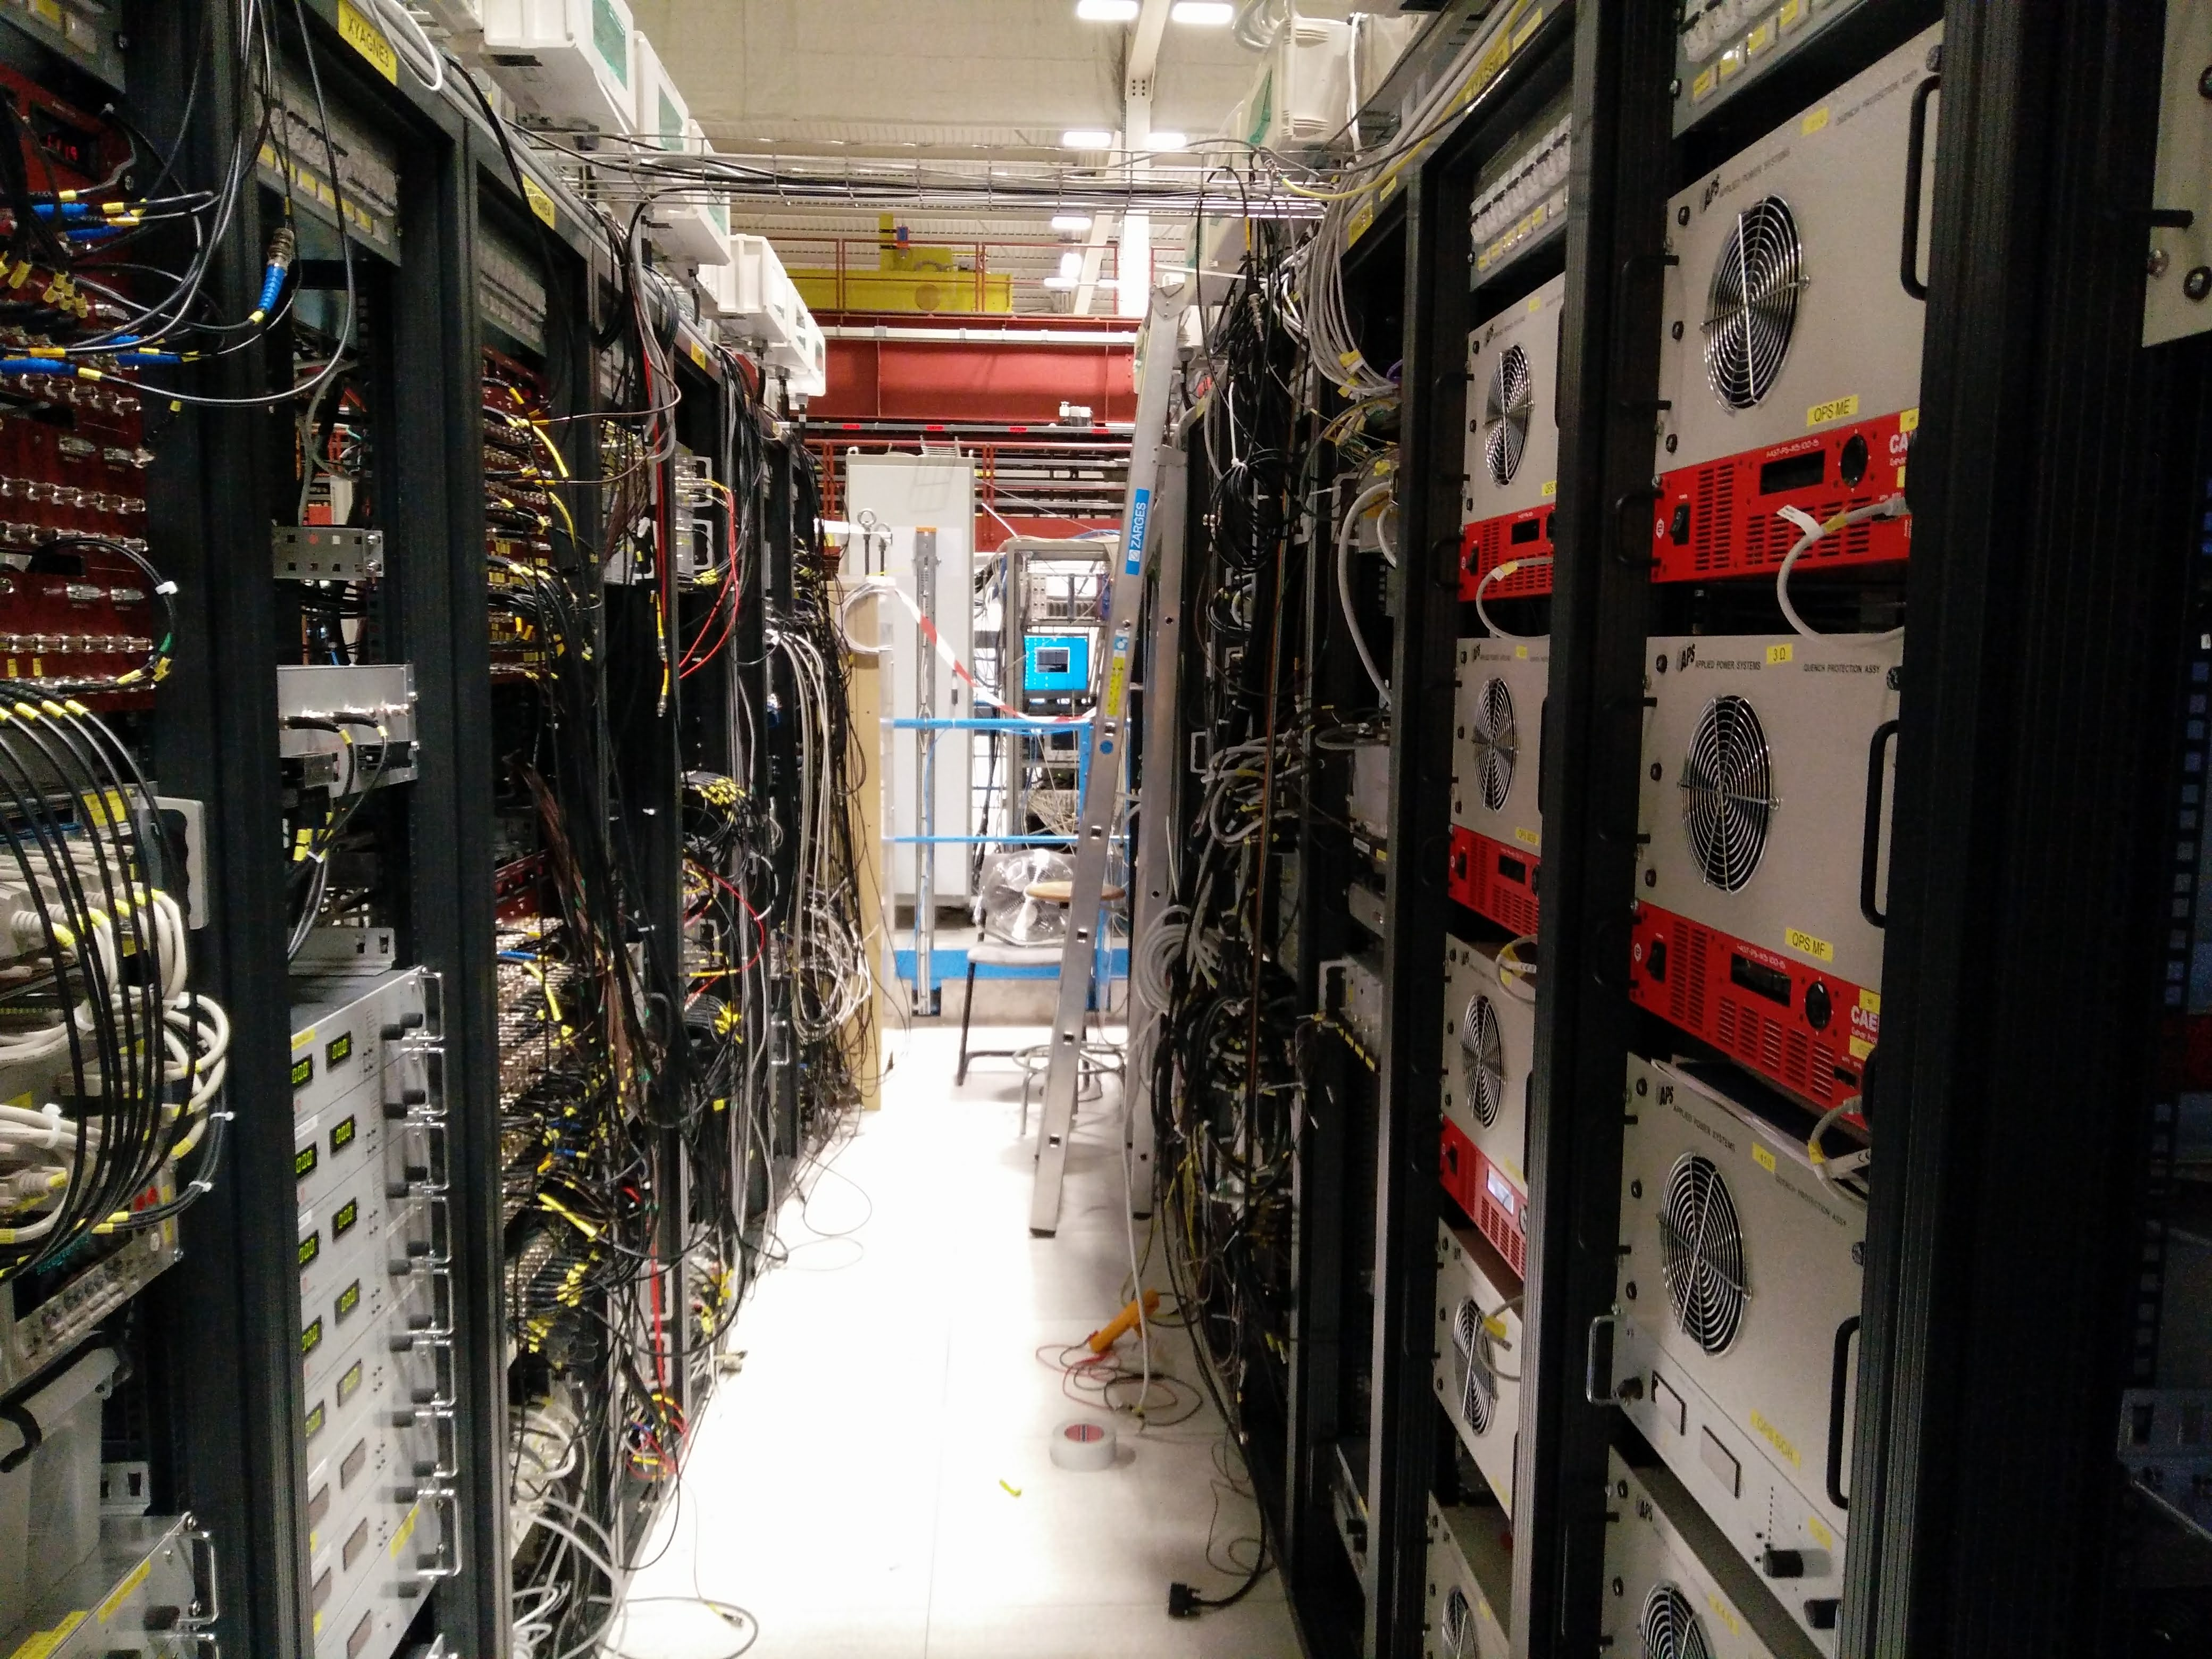
\includegraphics[width=80mm, height=50mm]{control_platform}
\caption{PCI 8430 card (left), and Computers on control platform equipted by DAQ cards (right) }
\end{figure}
	
\subsubsection{Virtual Instrument}

The Virtual Interface of VI that I have designed will contorl the valves, magnets, and vacuum pumps that are connected to the positron source and accumulator. You can see the front panel or the GUI of VI[figure???]. 

The block diagram that controls this VI consists of three different sub VIs. I have desinged  block diagram to be modular and mmy supervisor can add other control and options after my departure. each of these sub VIs is for Valves, Vacuum pumps and pass camra section. These VIs must feed by a number that indicates the state of valve or vacuum pump to be On or Off, and by a string that the Icon of the elents in GUI are in it. The sub VI will brrows the proper Icon considering the numeric input and will send the picture as Output. all of this elements are in a event structure to reduce the amount of cpu uccpation. the reduction of CPU use is because the while loop around the event structure will run for 1 time, just when you changfe the values of the each event structure.

\subsection{Compact Rio Upgrade}
As mentioned bofore, handling advanced experimnets requires advanced electronic setups. As the  time passes the electronics and computers get more powerful. So one of the important 'Must do's for every experiment is upgrading the componets of experiment to the last technologies. ALPHA was born at 2009[????] and since that day many updates had be done on setup and computers. A part of new update is transferring the old computers with DAQ cards to professional Compact Rio computers that are designed mainly for Experimnetal and data aquistion purposes. In more details, CompactRIO (or cRIO) is a real-time embedded industrial controller made by National Instruments for industrial control systems. The CompactRIO is a combination of a real-time controller, reconfigurable IO Modules (RIO), FPGA module and an Ethernet expansion chassis.[Wikipedia of cRio](figure \ref{crio}). In these computers we use DAQ madules instead of DAQ cards. This will make the control platform very compact and of course more professional. In some of the madules that we use with this compueters we need to seperate the data lines in order to use them individualy. for this purpose we need to design a printed circuit board (PCB), that maps every pin on D-subminature connector to individual lemo connectors.

\begin{figure}[h]
\centering
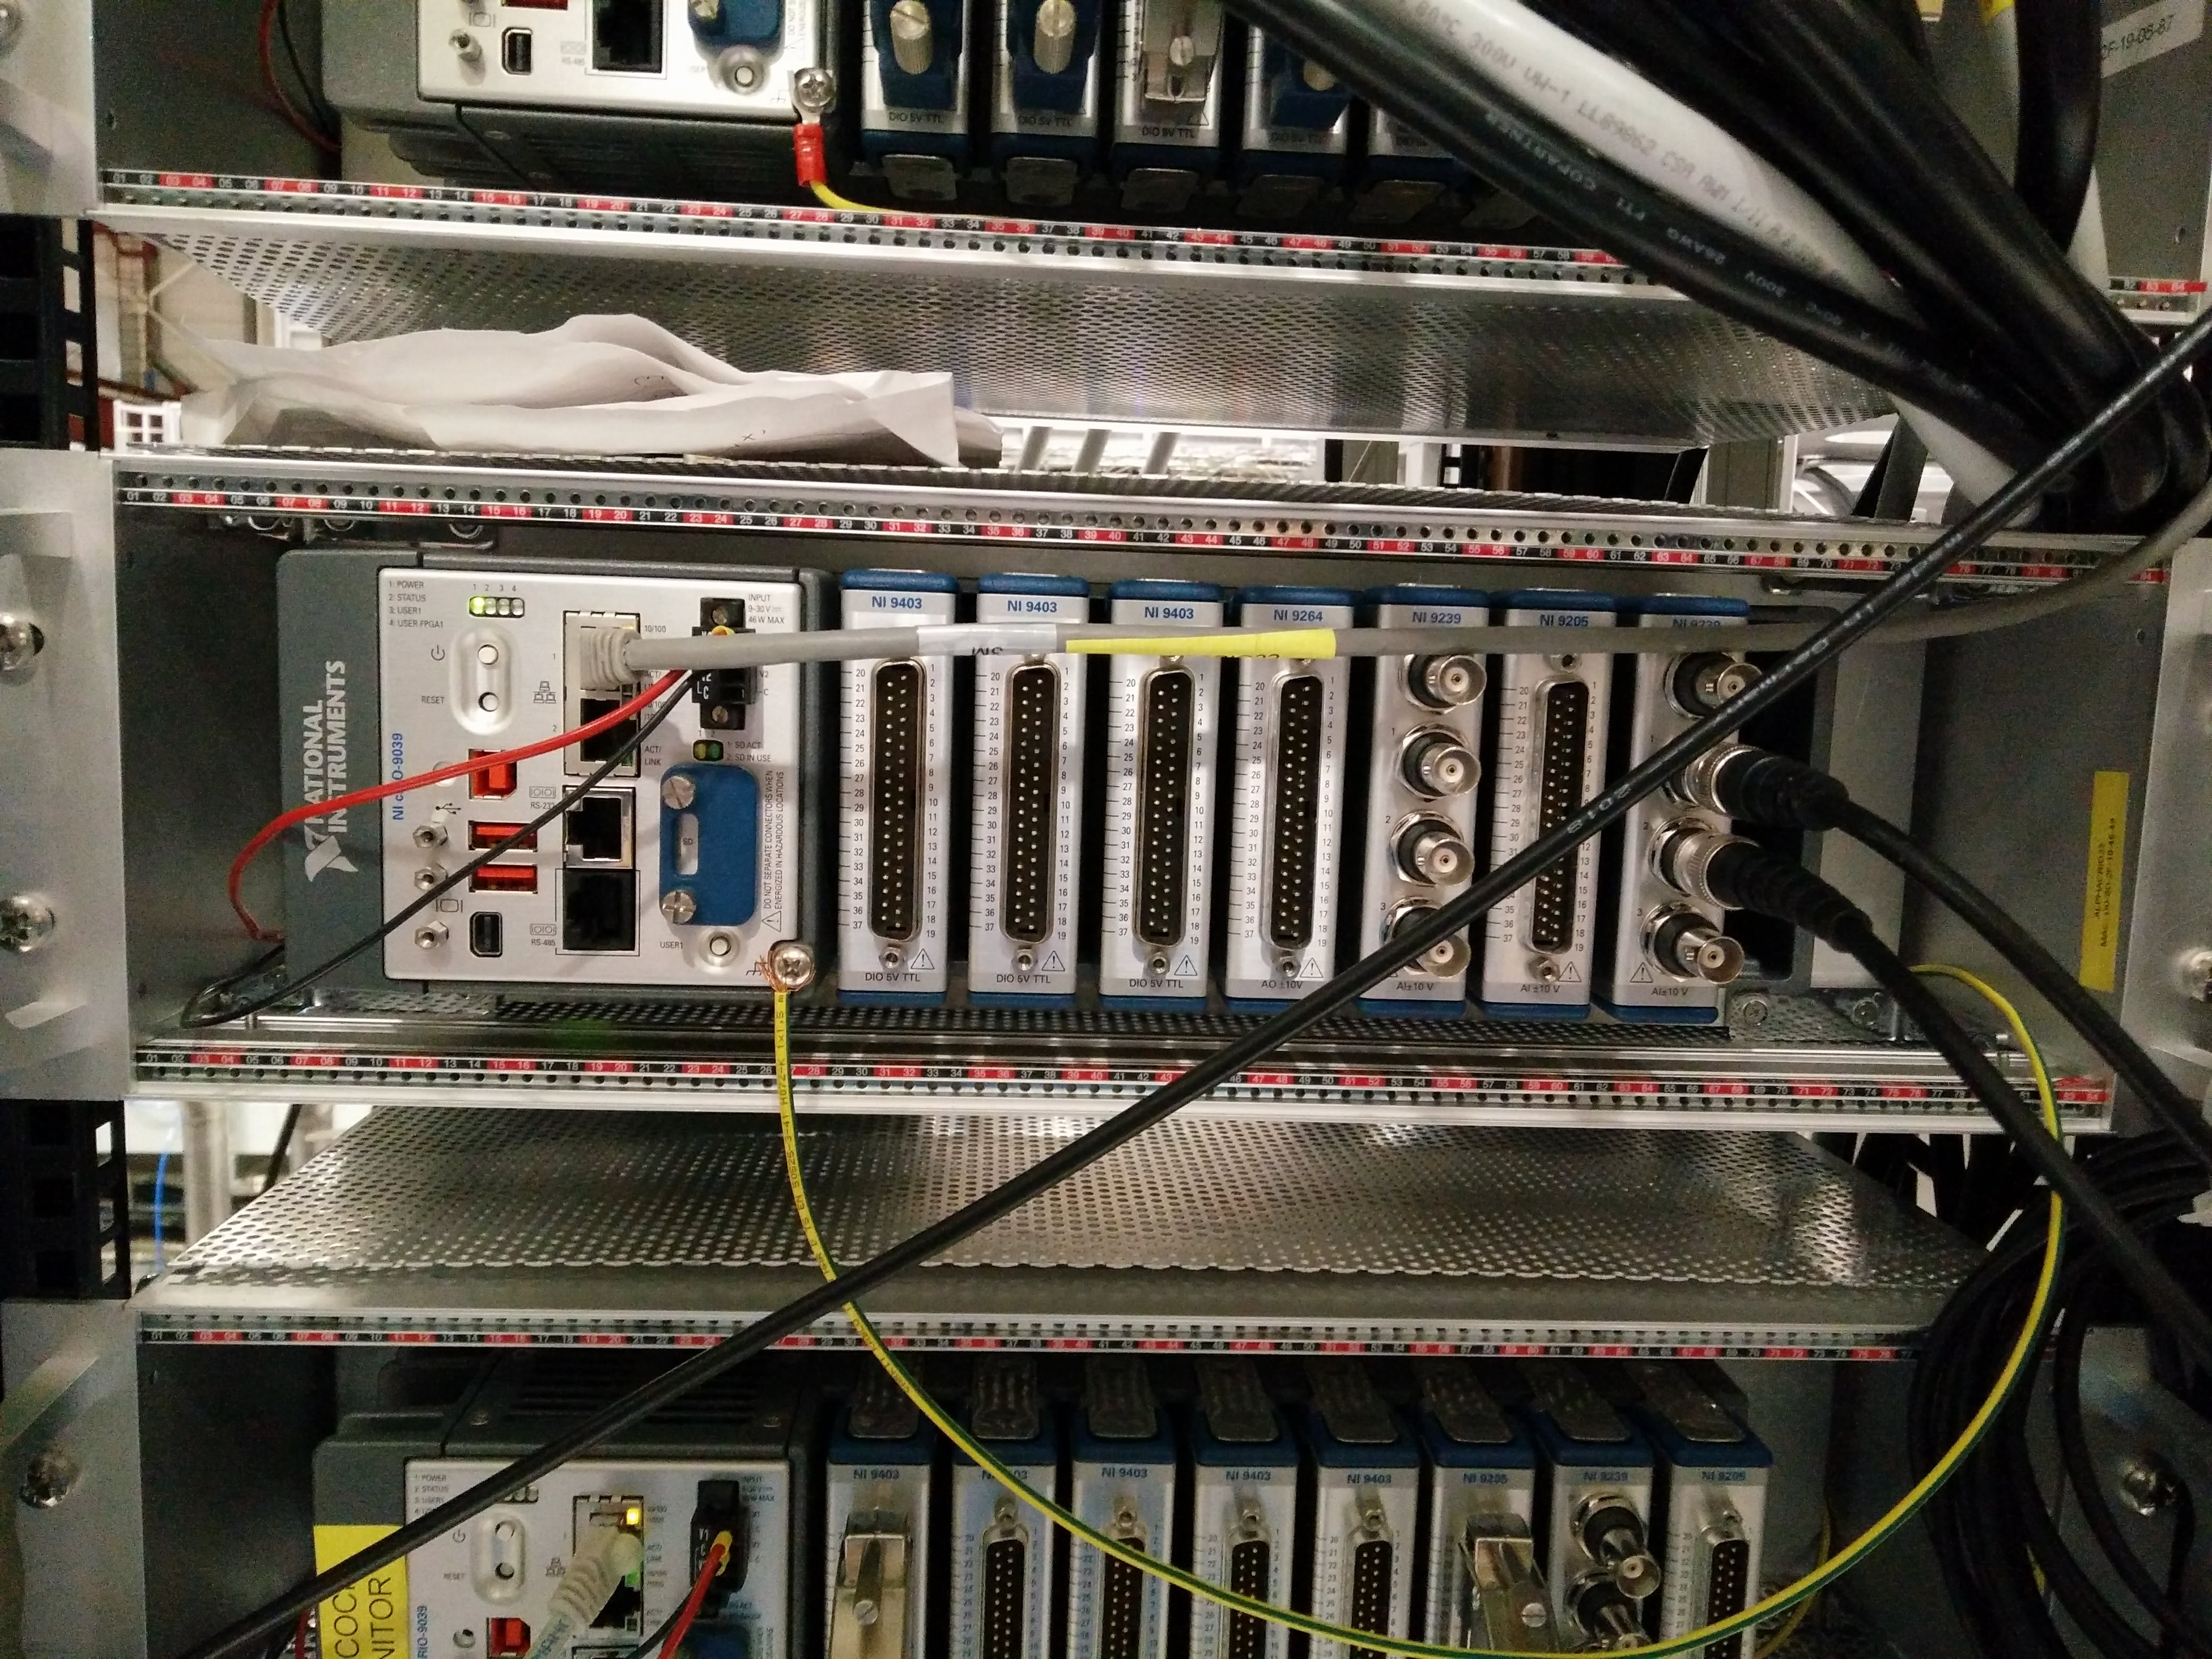
\includegraphics[width=105mm, height=60mm]{crio}
\caption{Compact Rio}
\label{crio}
\end{figure}

\subsubsection{PCB and Front Panel Design}
In this project I designed the PCB using "Altium design' software. this PCBs connect the D-subminator connector to individual Lemo Connectors. Throughout this report I will call these PCBs "Data Line Seperator" or DLS. We had four different types of madules, so I needed to design four differnet PCBs.
The madules was NI9264, NI9401, NI9403, NI9205. these madules are digital and analog madules that are connected to compact rio system to control the experiment aparues. For example one can control valvs, vacuum pumps, mass flow rate controlers, etc. These are done by using LabVIEW interface which I worked with and designed an interface in other project that  I will descripe later. You can find mentioned modules in figure \ref{mod}

\begin{figure}
\centering
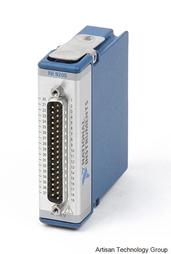
\includegraphics[width=27mm, height=37mm]{ni9205}
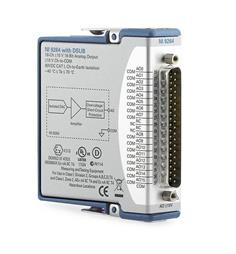
\includegraphics[width=27mm, height=37mm]{ni9264}
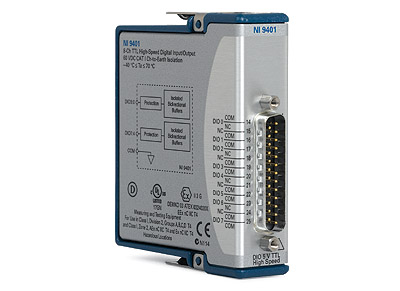
\includegraphics[width=38mm, height=37mm]{ni9401}
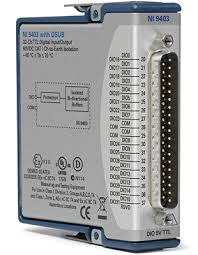
\includegraphics[width=24mm, height=37mm]{ni9403}
\caption{(left to right) NI 9205, NI 9264, NI 9401, NI 9403}
\end{figure}

As I said before, for complicated experiments there is a control platform that contols the parameters of experiment. For example figure ??? is the control platform of APLHA experiment.
These platforms are where that the Compact Rio will sit at. Each compact rio will be held at chassis and these chassises will be held horizontaly on top of each other by [sotoon]. so to keep every thing not messy, we need to design fron panels that can mount on chassies, and srew the PCBs to them. I did so for each of the modules and you can see the front panel of the NI9205 module in figure ???. You can find full documents at my github repository for cern as well.


\begin{figure}[h]
\centering
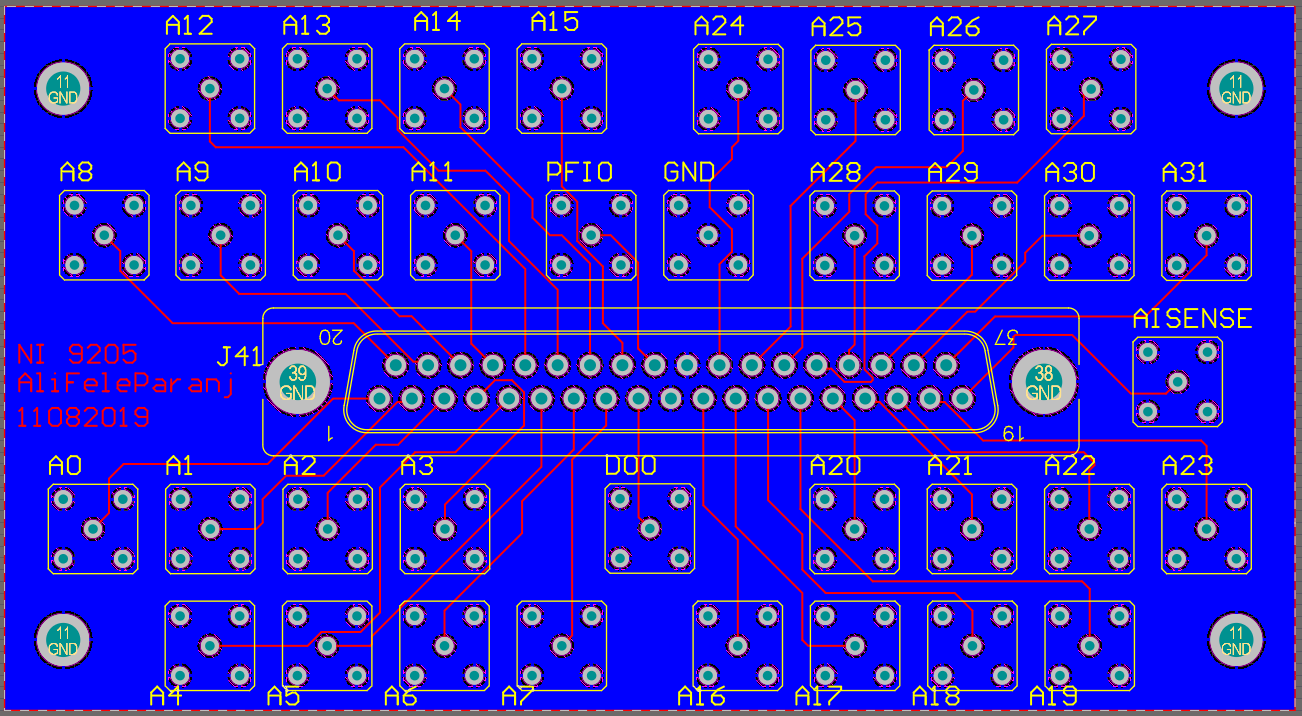
\includegraphics[scale=0.17]{ni9205_pcb}
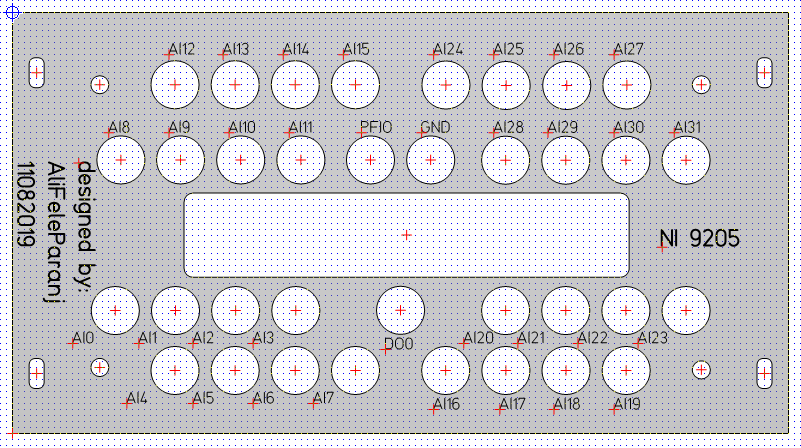
\includegraphics[scale=0.27]{ni9205panel}
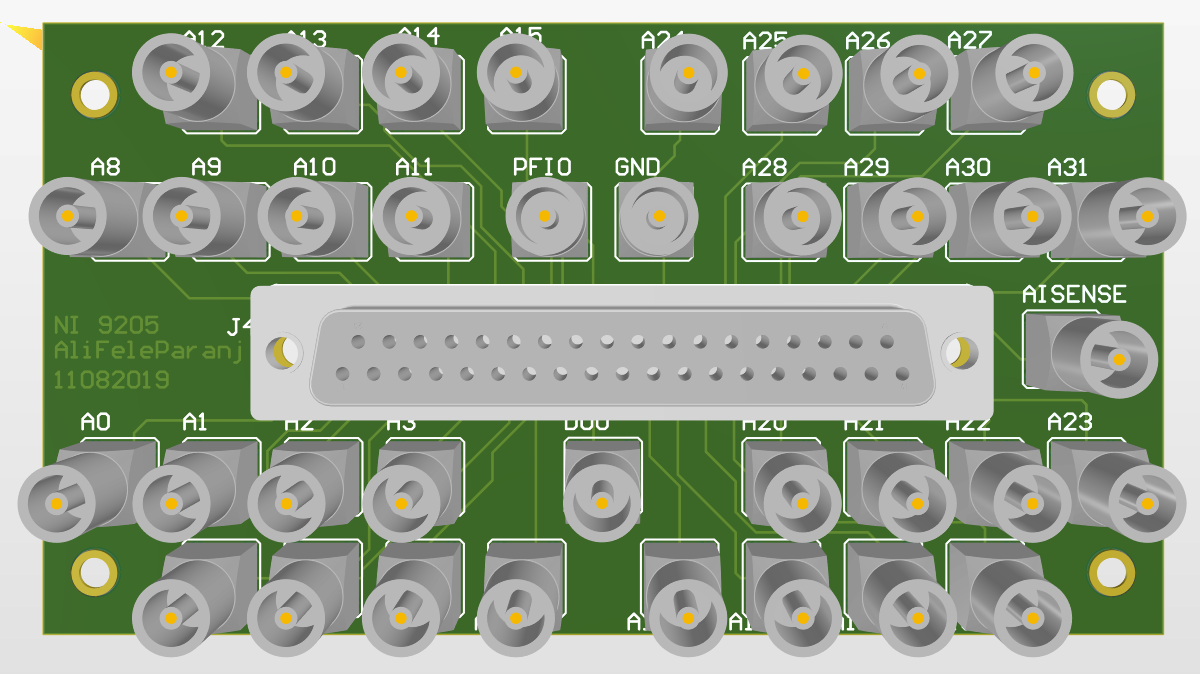
\includegraphics[scale=0.27]{ni9205_3d}
\caption{First: DLS designed for NI9205 module, Second: 3D model of DLS, Third: Front Panel Designed for NI9205 DLS}
\label{NI}
\end{figure}



\subsection{Full Simulation}
‌Simple simulations are very useful when you want to evaluate your stimates using the minimum computation resources. But after finding the rough simulations satisfactory, you need to improve you simulated model and add more details to it. In the simple simualtion of buncher we find out that buncher works pretty well in bunching the expanding beam. So we decided to add more details to our simulation and simulate the full setup of magnets and beam line.
\subsubsection{Geometry}
To make it possible, we needed to make a CAD model of magents in full setup. The data of magnets was in a file with .cond type which was designed to feed the data to the OPERA software to calculate the magnetic field. After finding the meaning of those numbers on .cond file with the help of my supervisor ,First I wrote a python code to transfer those data to a more clear data set of magnets[figure of excel]. Then I used the Inventor software to design all of the 82 magnets that contributes in the magnetic field of beam line. Then I added the Inventor model of buncher and Accumulator(that was previuosly created by ALPHA group).
\subsubsection{Running Simulation on HTCondor Provided by LXPLUS Linux Cluster}
Althogh I was using two computers in parallel to generate the results faster, but Since Simulating the full setup was very computational expensive, So it impossible to simulate the whole setup with 32 GB of RAM. The time of simulation was very long as well, so we needed to run our simulation on HTcondor. HTcondor  stands for High Throughput Computing and is a specialized workload management system for compute-intensive jobs. Like other full-featured batch systems, HTCondor provides a job queueing mechanism, scheduling policy, priority scheme, resource monitoring, and resource management. Users submit their serial or parallel jobs to HTCondor, HTCondor places them into a queue, chooses when and where to run the jobs based upon a policy, carefully monitors their progress, and ultimately informs the user upon completion[https://research.cs.wisc.edu/htcondor/description.html]. linux clusters of cern provides the HTcondor computation and you can access big memory nodes and higher number of cpu cores. But since I was here yat cern for 53 days, it was impossible to run all of the simulations on clusters and get results. So in this part of my project I set up the full simulation file with the real initial values used in apartues .since I was familiar with Linux I could set up the environement and submit some sample simularions [figure lxplus] and my supervisor will run the simulation on cluster after my departure. This simulation contains a parametric sweep to search the optimum values for "amplitude", "Frequency" and "phase" of the the sine potential that is applied on the buncher. The real Quantitive results will be generated with this simulation and it will help us to tune the paramters of bunher on order to bunch the positron beam.

\begin{figure}
\centering
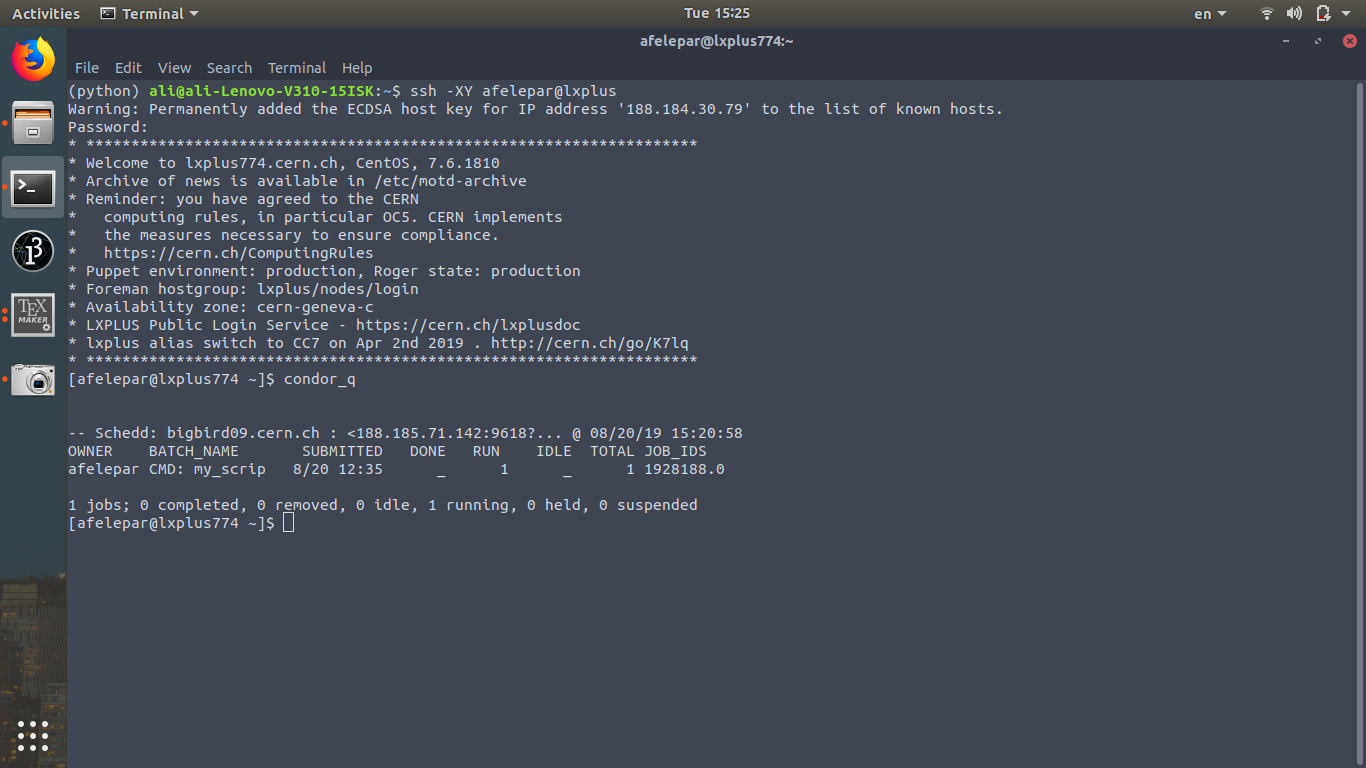
\includegraphics[scale=0.25]{lxplus}
\caption{SSH tunnel to lxplus cluster through linux terminal on my laptop}
\end{figure}


\section{Lectures, Workshops and Visits}
During my stay at cern I attended almost all of the Lectures. This lecture series was one of the best ones I attended during my life. The content of lectures was very interesting, the presentation of the lecturers was excellent and the lectures was very up to date. Here is the Courses that I attended and the "Physics and Medical Applications" I think was the best among them which was the most relevant subject to my field of studies.
\subsection{Classroom Courses}

\begin{enumerate}

\item Physics and Medical Applications by Manjiy Dosanjih
\item Particle World by Tara Shears
\item Detectors by Werner Riegler
\item Foundation of Statistics by Nicolas Berger
\item Electronics DAQ and Trigger
\item Theoretical Concepts in Particle Physics by Andrew Cohen
\item From Raw Data to Physics Results by Paul James
\item Experimental Physics at Hadron Colliders by Marumi Kado
\item The Standard Model
\item Astroparticle Physics
\item Heavy Ions
\item Introduction to Cosmology
\item Beyond Standard Model
\item Nuclear Physics at CERN
\item What is String Theory
\item Future High-Energy Collider Projects
\item Antimatter at Lab

\end{enumerate}


\subsection{Online Courses}
I attendent some Online safety courses which was as following :

\begin{enumerate}
\item Computer Security
\item Emergency Evacualtion
\item Radiation Protection
\item Electrical Safety Fundamentals
\item Electrical Safety Facilities
\item Cryogenic Safety Awarness
\item Chemical Safety Awarness
\end{enumerate}

\subsection{Workshops and Visits}
During the program there was many cool workshops and visits. Here is a list of items that I attended

\begin{enumerate}

\item Open Data in Educational Activities Workshop
\item Basic Cloud Chamber Workshop
\item Advanced Cloud Chamber Workshop
\item Data Acquistion / Trigger Workshop
\item Root Summer Student Workshop
\item Silicon Senors
\item CMS visit
\end{enumerate} 







\end{document}